\subsection{脉冲发生模块动力学模型及频率响应特性研究}
\subsubsection{脉冲发生模块流体-固体耦合机制及受力分析}

如图\ref{fig:working_cycle_pulse_module}所示，脉冲发生模块的工作工况主要分为四个阶段：

\begin{itemize}
	\item 蓄能阶段：当高压流体经由钻柱进入脉冲发生模块芯轴腔室时，由于侧向出水孔处于关闭状态，下方长开喷嘴具有节流效果，流体经过活塞腔入水孔进入腔室，腔室形成半封闭空间。随着泵入流量 的持续补充，流体被压缩，腔内静压力  迅速升高。
	\item 开启阶段：当液压力作用在活塞端面产生的推力超过弹簧预紧力及摩擦力之和时，活塞克服阻力向开启方向位移。当位移达到设计临界点 时，出水孔打开，活塞从出水孔打开处向上运动至最远点（速度为零处）。
	\item 喷射阶段：腔内高压流体瞬间经喷头排出，形成高速脉冲射流冲击井筒环空，活塞从最远点返回至侧向出水孔。 
	\item 复位阶段： 随着压力下降，弹簧势能释放，驱动活塞迅速复位至初始位置，关闭出水孔，系统进入下一个循环。
\end{itemize}

\begin{figure}[htbp]
	\centering
	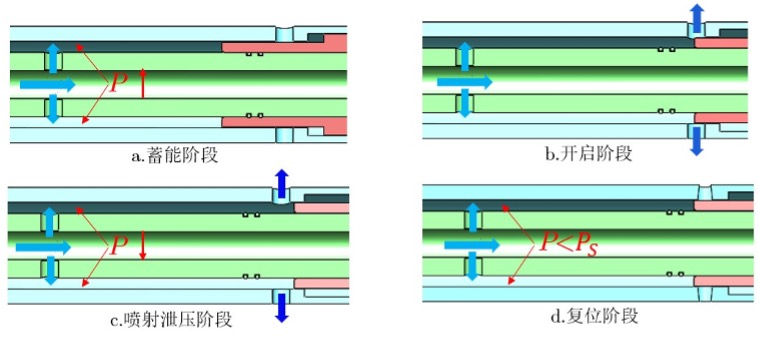
\includegraphics[width=0.9\textwidth]{figure/chapter3/working-cycle-pulse-module.jpg}
	\caption{脉冲发生模块工作周期示意图}
	\label{fig:working_cycle_pulse_module}
\end{figure}

（1）往复活塞受力模型

在活塞工作的任意周期瞬时$t$，往复活塞的运动状态取决于多种力场的综合作用—包括液压驱动力$F_p$，惯性力$F_a$，弹簧线性约束力$F_s$，粘性与摩擦阻力$F_d$。为了精确描述其动力学行为，建立如下受力平衡模型。

\begin{figure}[htbp]
	\centering
	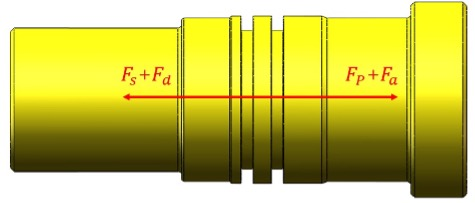
\includegraphics[width=0.6\textwidth]{figure/chapter3/force-analysis-reciprocating-piston.jpg}
	\caption{脉往复活塞受力分析图}
	\label{fig:force_analysis_reciprocating_piston}
\end{figure}

流体压力作用于活塞环形端面$A_1$。由于井下环境存在环空压力$P_{out}$，有效驱动力表现为内外压差：
\begin{equation}
	F_p(t)=\left[P(t)-P_{out}\right]\cdot A_1
\end{equation}
式中，$A_1$为活塞有效受压面积，其计算公式为：
\begin{equation}
	A_1=\frac{\pi}{4}\left(r_1^2-r_2^2\right)
\end{equation}
式中，$r_1$为活塞腔外径，m；$r_2$为活塞腔内径，m；

本装置采用高刚度矩形截面螺旋弹簧作为复位元件，在同等安装空间下可提供更大的恢复力，且其刚度特性受截面长宽比影响显著。根据材料力学及弹簧设计理论，矩形截面弹簧的等效刚度$k$可表征为：
\begin{equation}
	k=\frac{G\cdot b\cdot h^3}{n\cdot D^3} \eta
\end{equation}
式中，$G$为弹簧材料的弹性模量，Pa；

$b$为弹簧截面的径向宽度；

$h$为截面轴向高度；

$D$为弹簧的中径；

$n$为有效圈数；

$\eta$为形状修正系数，取决于长宽比$b/h$。

在脉冲发生模块工作过程中，弹簧力$F_s$随活塞位移$x(t)$呈线性变化关系：
\begin{equation}
	F_s(x)=k\cdot\left[x(t)+x_0\right]
\end{equation}

活塞在往复运动中受到密封件的干摩擦力$F_f$以及流体层间剪切产生的粘性阻尼力。为简化计算，通常采用等效粘性阻尼模型：
\begin{equation}
	F_d(t)=C\frac{dx(t)}{dt}
\end{equation}
式中，$C$为摩擦等效阻尼系数。

由于活塞在液体中高频振荡，会带动周围部分流体共同运动，从而产生惯性力$F_a$：
\begin{equation}
	F_a(t)=m\frac{d^2x(t)}{dt^2}
\end{equation}
式中，$m$为活塞及所有随动运动件的等效总质量，kg。

（2）流固耦合响应特性分析

脉冲发生模块的工作过程包括芯轴内腔的非稳态流场以及活塞运动两个方面，系统的动力学行为由流体压力场的变化与活塞的机械响应共同决定。

\begin{figure}[htbp]
	\centering
	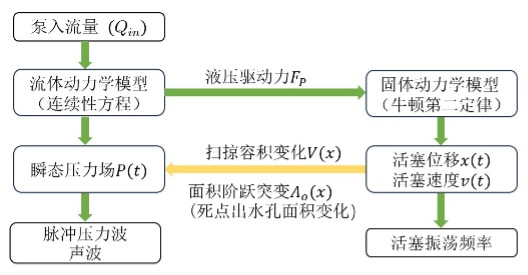
\includegraphics[width=0.7\textwidth]{figure/chapter3/FSI-logic.jpg}
	\caption{水力脉冲冲砂洗井工具脉冲发生模块结构图}
	\label{fig:FSI_logic}
\end{figure}

在脉冲循环中，流体与固体的相互作用主要体现在以下两个维度：

(1)压力对运动的驱动：随泵入流量$Q_{\mathrm{in}}$的积聚，腔室内流体被压缩，产生的瞬态压力$P(t)$作用于活塞端面$A_1$，形成驱动力$F_p$。当该力克服矩形弹簧预紧力及摩擦阻力后，改变活塞的运动状态。

(2)运动对压力的反馈：活塞的轴向位移$x$实时改变腔室的控制容积$V(t)$。当位移超过开启阈值$L$时，出水孔有效过流面积$A_o(x)$发生阶跃式变化，导致腔内流体迅速外泄，压力场随之重构。

系统的非线性特征主要源于开启时刻流道边界的突变。在活塞位移$x<L$时，系统处于蓄能阶段，流体处于高压状态；当$x>L$时，出水孔由封闭转为开启，系统边界由静态边界转变为自由出流边界。此时，活塞的往复运动会产生扫掠容积$A\cdot dx/dt$。在泄压阶段，活塞在矩形弹簧作用下迅速复位，其扫掠容积的方向与流体泄出方向相反，这种容积补偿效应是腔内形成瞬时负压物理过程的重要成因。

从能量角度分析，连续的流体压力能首先转化为弹簧的弹性势能与活塞的动能。在开启瞬间，由于矩形弹簧的高刚度特性，存储的能量在极短时间内释放，通过侧向出水孔转化为高速射流。这一过程伴随着剧烈的压力脉动，实现了对套管内壁及砂砾再沉积的振荡剥离。


\subsubsection{脉冲发生模块瞬态动力学模型构建}
在明确了脉冲发生模块内部流体与固体部件相互作用的物理机制后，为了能够定量分析脉冲发生模块在一个周期内活塞位移、速度随时间的变化关系，必须建立一套能够反映系统真实运动状态的数学模型。
根据流体连续性方程：

\begin{equation}
	Q = A_1\frac{dx}{dt}+Q_n
\end{equation}
式中，$A_1dx/dt$为用于推动活塞向上运动的体积变化率；$Q_n$为节流排量，$m^3/h$。

根据流体力学中的薄壁小孔流出模型，流经节流喷嘴的流量$Q_n$与缸内外压差$P(t)-P_{out}$的关系为
\begin{equation}
	Q_n=C_dA_n\frac{2(P(t)-P_{out})}{\rho_w}
\end{equation}
式中：$C_d$为喷嘴的流量系数，$A_n$为节流喷嘴的截面积，$m^2$，$\rho_w$为流体密度，$kg/m^3$。

由于$Q>>A_1\frac{dx}{dt}$，活塞运动对系统总流量的扰动微乎其微。将$Q_n$代入，则
\begin{equation}
	P(t)-P_{out}=\Delta P_{close}
\end{equation}


液压驱动力：
\begin{equation}
	\left(P(t)-P_{out}\right)\cdot A_1=\frac{A_1\rho_2}{2C_d^2A_n^2}Q^2
\end{equation}
取活塞初始静止位置为原点，其向下运动方向为正。活塞蓄能阶段的运动微分方程为：
\begin{equation}
	\frac{d^2}{dt^2}+C_1\left(\frac{dx}{dt}\right)^2+\left(C_2 x+C_3\right)\frac{dx}{dt}+C_4 x+ C_5 =0
\end{equation}

式中， $C_1$为非线性阻力系数，物体在流体中高速运动时，会产生与速度平方成正比的阻力：
\begin{equation}
	C_1=\frac{C_DA_2\rho_w}{2V\rho_f}
\end{equation}
$C_2$与$C_3$为粘性摩擦力阻尼，活塞与缸体之间存在微小的环空狭缝，当活塞运动时，流体在狭缝中产生剪切流动，这个摩擦力与运动速度成正比
\begin{equation}
	C_2=-\frac{2\mu\pi r_1}{\rho_f V\delta}
\end{equation}
\begin{equation}
	C_3=\frac{2\mu\pi\left(l_1r_1+l_2r_2\right)}{\rho_f V \delta}
\end{equation}
$C_4$为弹簧刚度与静水压恢复项：
\begin{equation}
	C_4=\frac{K}{\rho_f V}-\frac{\pi r_1 g \delta \rho_w}{\rho_f V}
\end{equation}
 $C_5$为常数驱动力项，不随时间、位移和速度改变：
 %这儿没写完
 
 式中：$r_1$为活塞腔外径，$m$；$r_2$为活塞腔内径，$m$；$C_D$为量纲阻力系数,它随着物体的形状和雷诺数而变，流体作用于流体的阻力大小与其成正比；$\rho_w$为流体密度，$kg/m^3$；$\rho_f$为活塞密度，$kg/m^3$；$K$为弹簧刚度，$N/m$；$V$为活塞体积，$m^3$；$\delta$为活塞与缸体之间的间隙，$m$；$l_1$为从侧向出水孔到活塞下端距离，$m$；$l_2$为活塞总长度，$m$；$\mu $，流体粘度，$Pa\cdot s$；$g$为重力加速度，$m/s^2$。
 
 活塞开启阶段的运动微分方程为：
 
 式中：
 
 %有两个方程没写出来。
 
 其中：当活塞位移到侧向出水流孔打开时，此时流体有了两条并行的通道：节流喷嘴$A_n$和侧向出水孔孔（设其流通面积为$A_h$）。由于总泄流面积增加，系统压力瞬间卸载，导致压差下降：
 %这里缺一个方程
 
 活塞喷射阶段的运动微分方程为：
  %这里缺一个方程
  
  式中：
  %这里缺一个方程
  %这里缺一个方程
活塞复位阶段的运动微分方程为：

%这里缺一个方程

式中：


把四个阶段活塞的运动微分方程联立：


活塞各个运动阶段所满足的初始条件分别为：

式中：$h$为侧向出水孔距活塞下端的距离，$\mathrm{m}$；$h_1$为活塞运动的最高点高度，$\mathrm{m}$；$v_1$为上升时活塞运动到侧向出水孔处的速度，$\mathrm{m/s}$；$v_2$为下降时活塞运动到侧向出水孔处的速度，$\mathrm{m/s}$。

根据上述模型及定解条件即可确定出脉冲发生模块的脉冲周期,以及在脉冲过程中任意时刻活塞的运动速度、位置等参数[68-69]。

本节通过研究了脉冲发生模块内部流场与固体组件受力特性，构建了描述其动力学行为的非线性常微分方程组。该模型以活塞运动微分方程为核心，联立腔室流体连续性方程，定量刻画了泵入流量 、下接头喷嘴泄流 以及矩形弹簧刚度对脉冲频率的协同作用机制，为后续揭示结构参数对系统振荡频率奠定了严谨的数学基础。

\subsubsection{关键设计参数对脉冲发生模块动力学特性的影响规律}

为验证系统非线性动力学模型的准确性，并揭示脉冲发生模块的瞬态运动规律，提取排量$Q=50\mathrm{m^3/h}$，侧向出水孔高度$l_1=75\mathrm{mm}$，弹簧刚度$K=757176\mathrm{N/m}$下活塞位移与速度随时间的响应特性曲线。

如图\ref{fig:piston_displacement_VS_time}所示，活塞从初始位置($x=0$)启动，在节流喷嘴产生的节流压差作用下加速向下运动，在$t=6.08\mathrm{ms}$时，活塞位移达到$75\mathrm{mm}$(侧向出水孔位置)，该阶段耗时约占整个周期的47.3（单位是什么）。活塞越过$75\mathrm{mm}$刻度线后，侧向出水孔打开，缸内流体压力骤降导致主驱动力消失，活塞在复位弹簧的作用下减速。在$t=7.75\mathrm{ms}$时，活塞速度降至零，活塞唯一达到整个周期最大冲程$88.13\mathrm{mm}$。活塞在最大冲程处复位，由被压缩的弹簧释放弹性势能驱动其向上回程。在$t=9.44\mathrm{ms}$时，活塞向上退回并再次经过$75\mathrm{mm}$位置，由于伴随有残余液压力及向下的重力阻碍，回弹段的曲线斜率略低于下击段。活塞向上越过侧向出水孔致其关闭，缸内瞬间重新憋起高压，形成液压阻力。 在$t=12.86\mathrm{ms}$时，活塞回落至$0\mathrm{mm}$的初始位置。从位移响应曲线可知，在 $Q=50\mathrm{m^3/h}$排量下，系统单次工作周期为$12.86\mathrm{ms}$，对应的工作频率为$77.76\mathrm{Hz}$。

\begin{figure}[htbp]
	\centering
	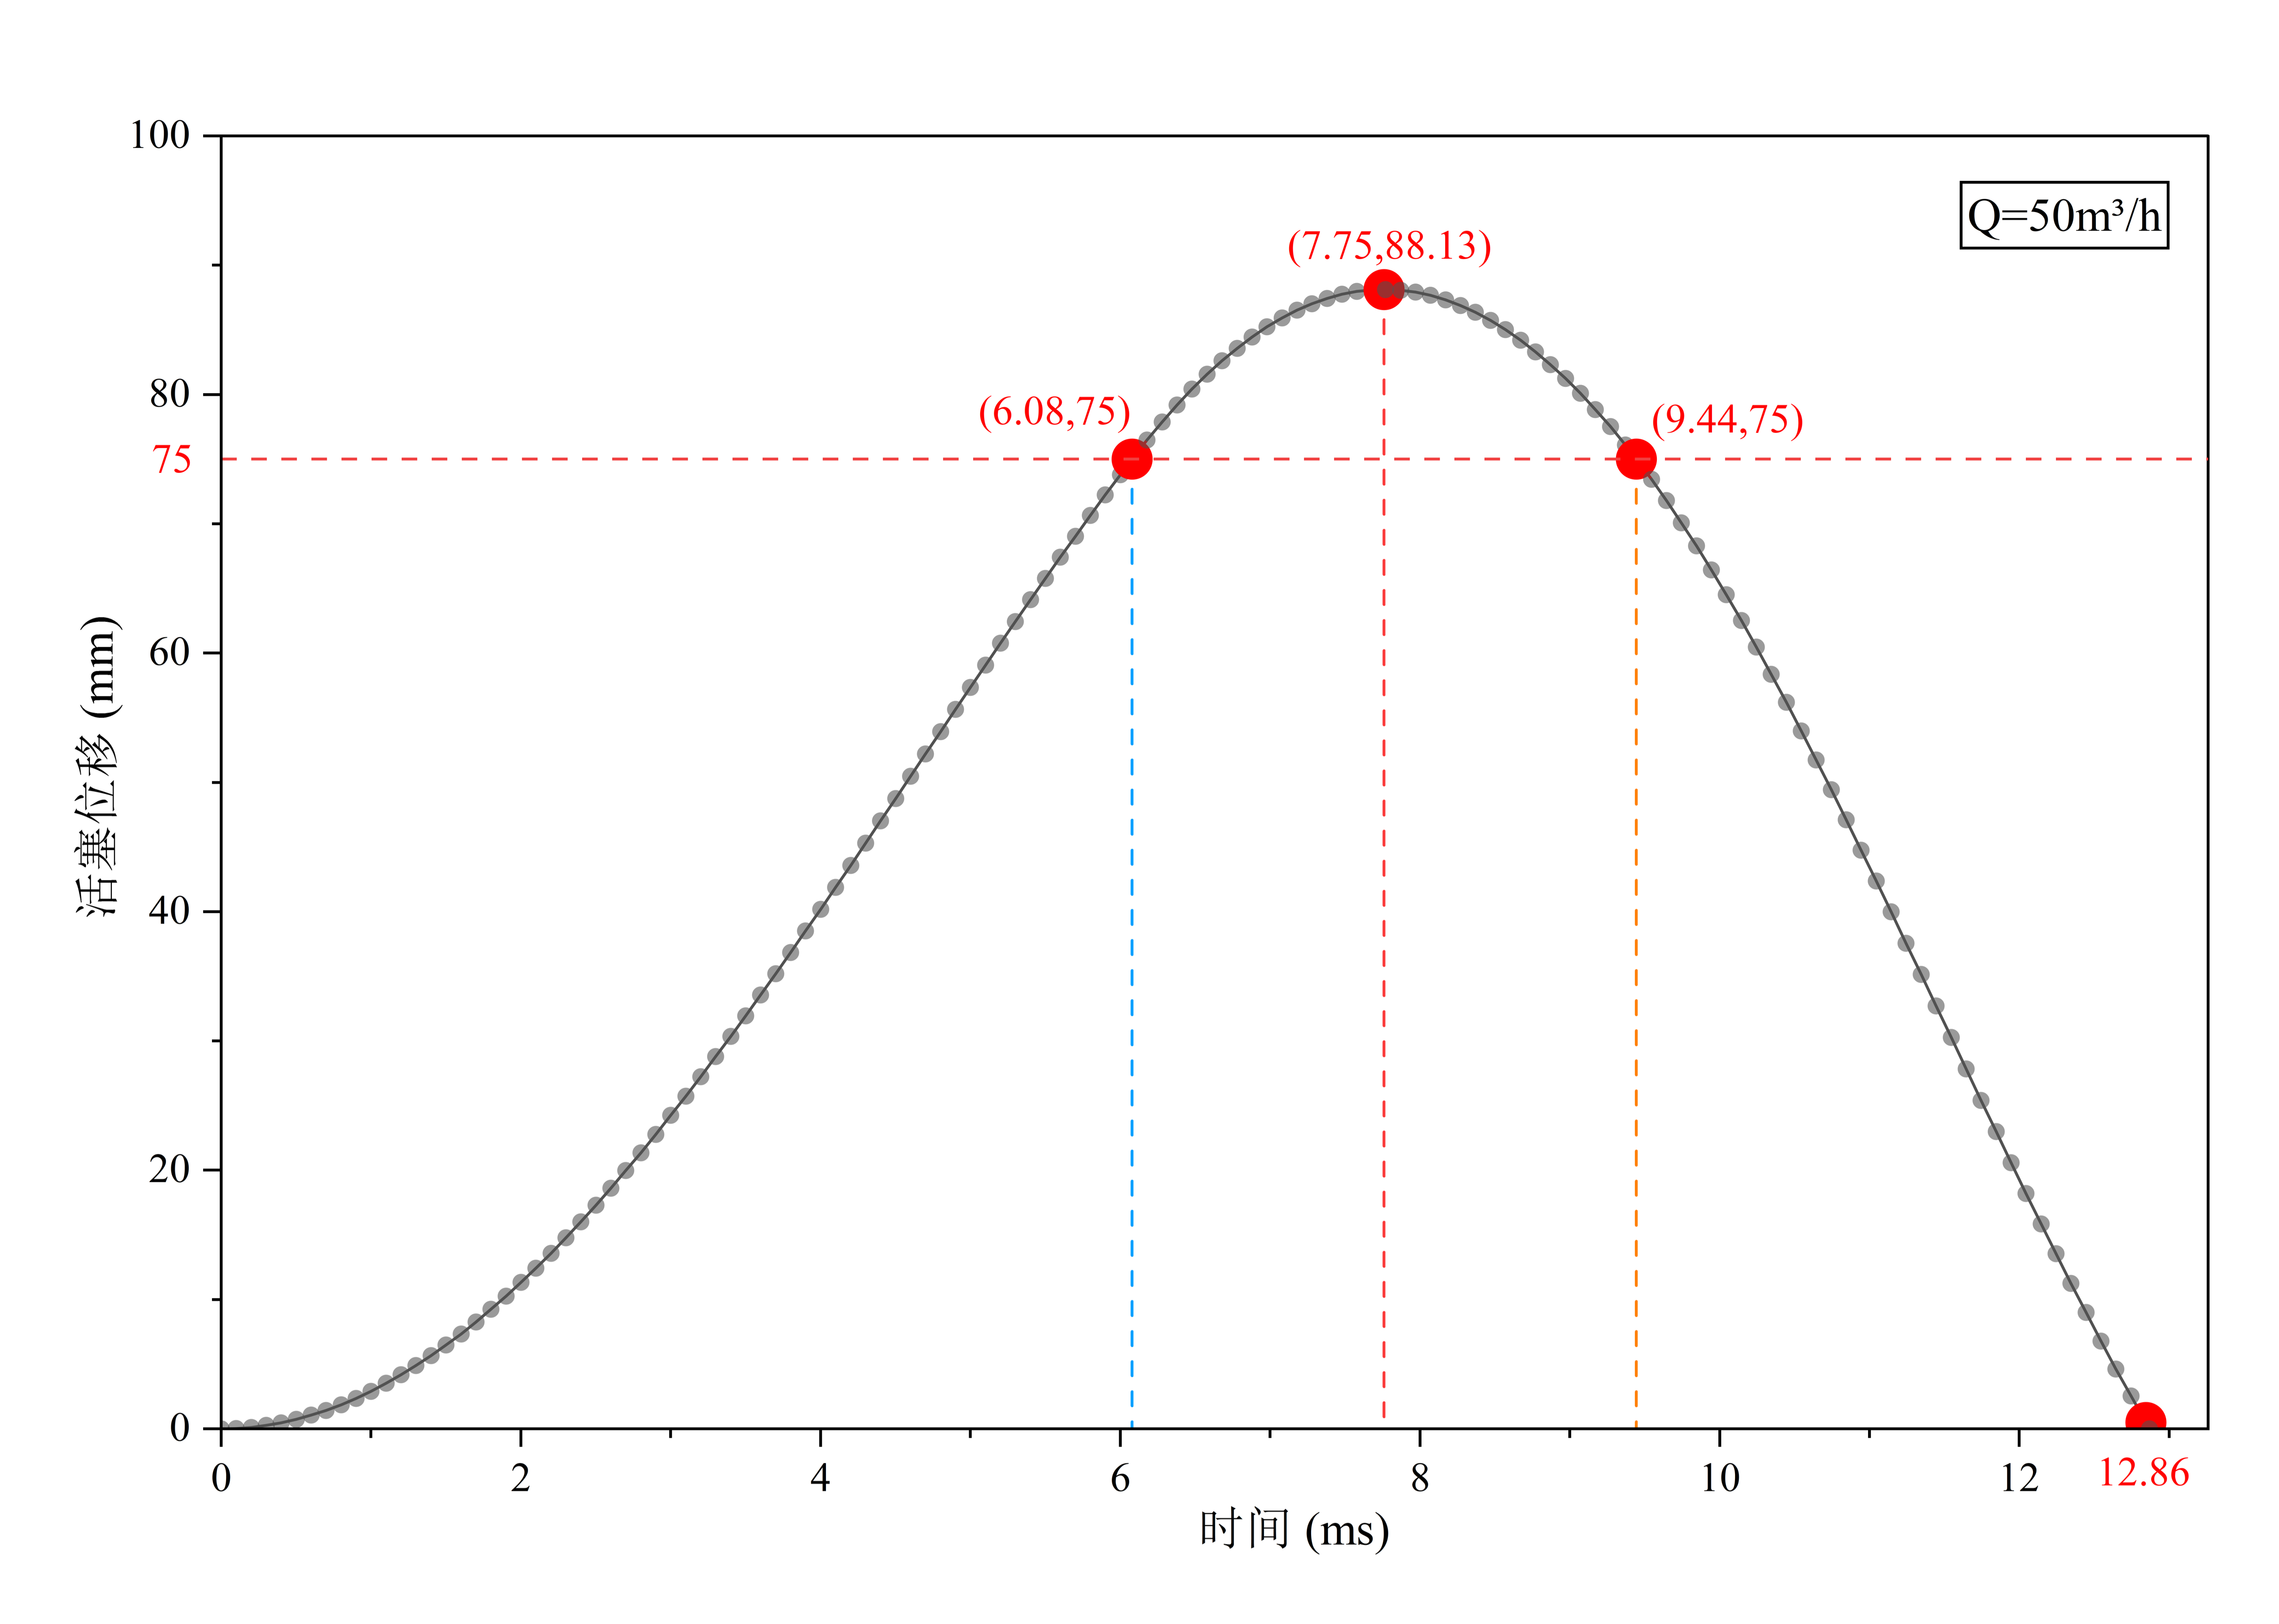
\includegraphics[width=0.7\textwidth]{figure/chapter3/piston-displacement-VS-time.png}
	\caption{活塞位移随时间变化曲线}
	\label{fig:piston_displacement_VS_time}
\end{figure}

如图\ref{fig:piston_velocity_VS_time}所示，活塞启动后，在压差作用下速度迅速增加，在$t=4.6\mathrm{ms}$时，活塞正向速度达到最大$17.26\mathrm{m/s}$。之后，由于弹簧被压缩，弹簧的弹性恢复力使活塞开始减速，在$t=6.08\mathrm{ms}$时，速度曲线的斜率出现了一个极其明显的折点， 标志着侧向出水孔被瞬间触发打开。液压驱动力发生减小，系统加速度突变为极大的负值。在纯机械弹簧力的强力压迫下，活塞速度在$1.68\mathrm{ms}$内从十多米每秒骤降至零，$t=7.75\mathrm{ms}$到达冲程死点）。经过下死点后，活塞速度变为负值（活塞向上运动），负向速度持续攀升，并在$t=11.44\mathrm{ms}$时刻达到整个周期的速度绝对值极值$-24.37\mathrm{m/s}$。在达到最大负向速度后，曲线斜率发生偏折，速度在初始限位和压差的作用下降为零。

\begin{figure}[htbp]
	\centering
	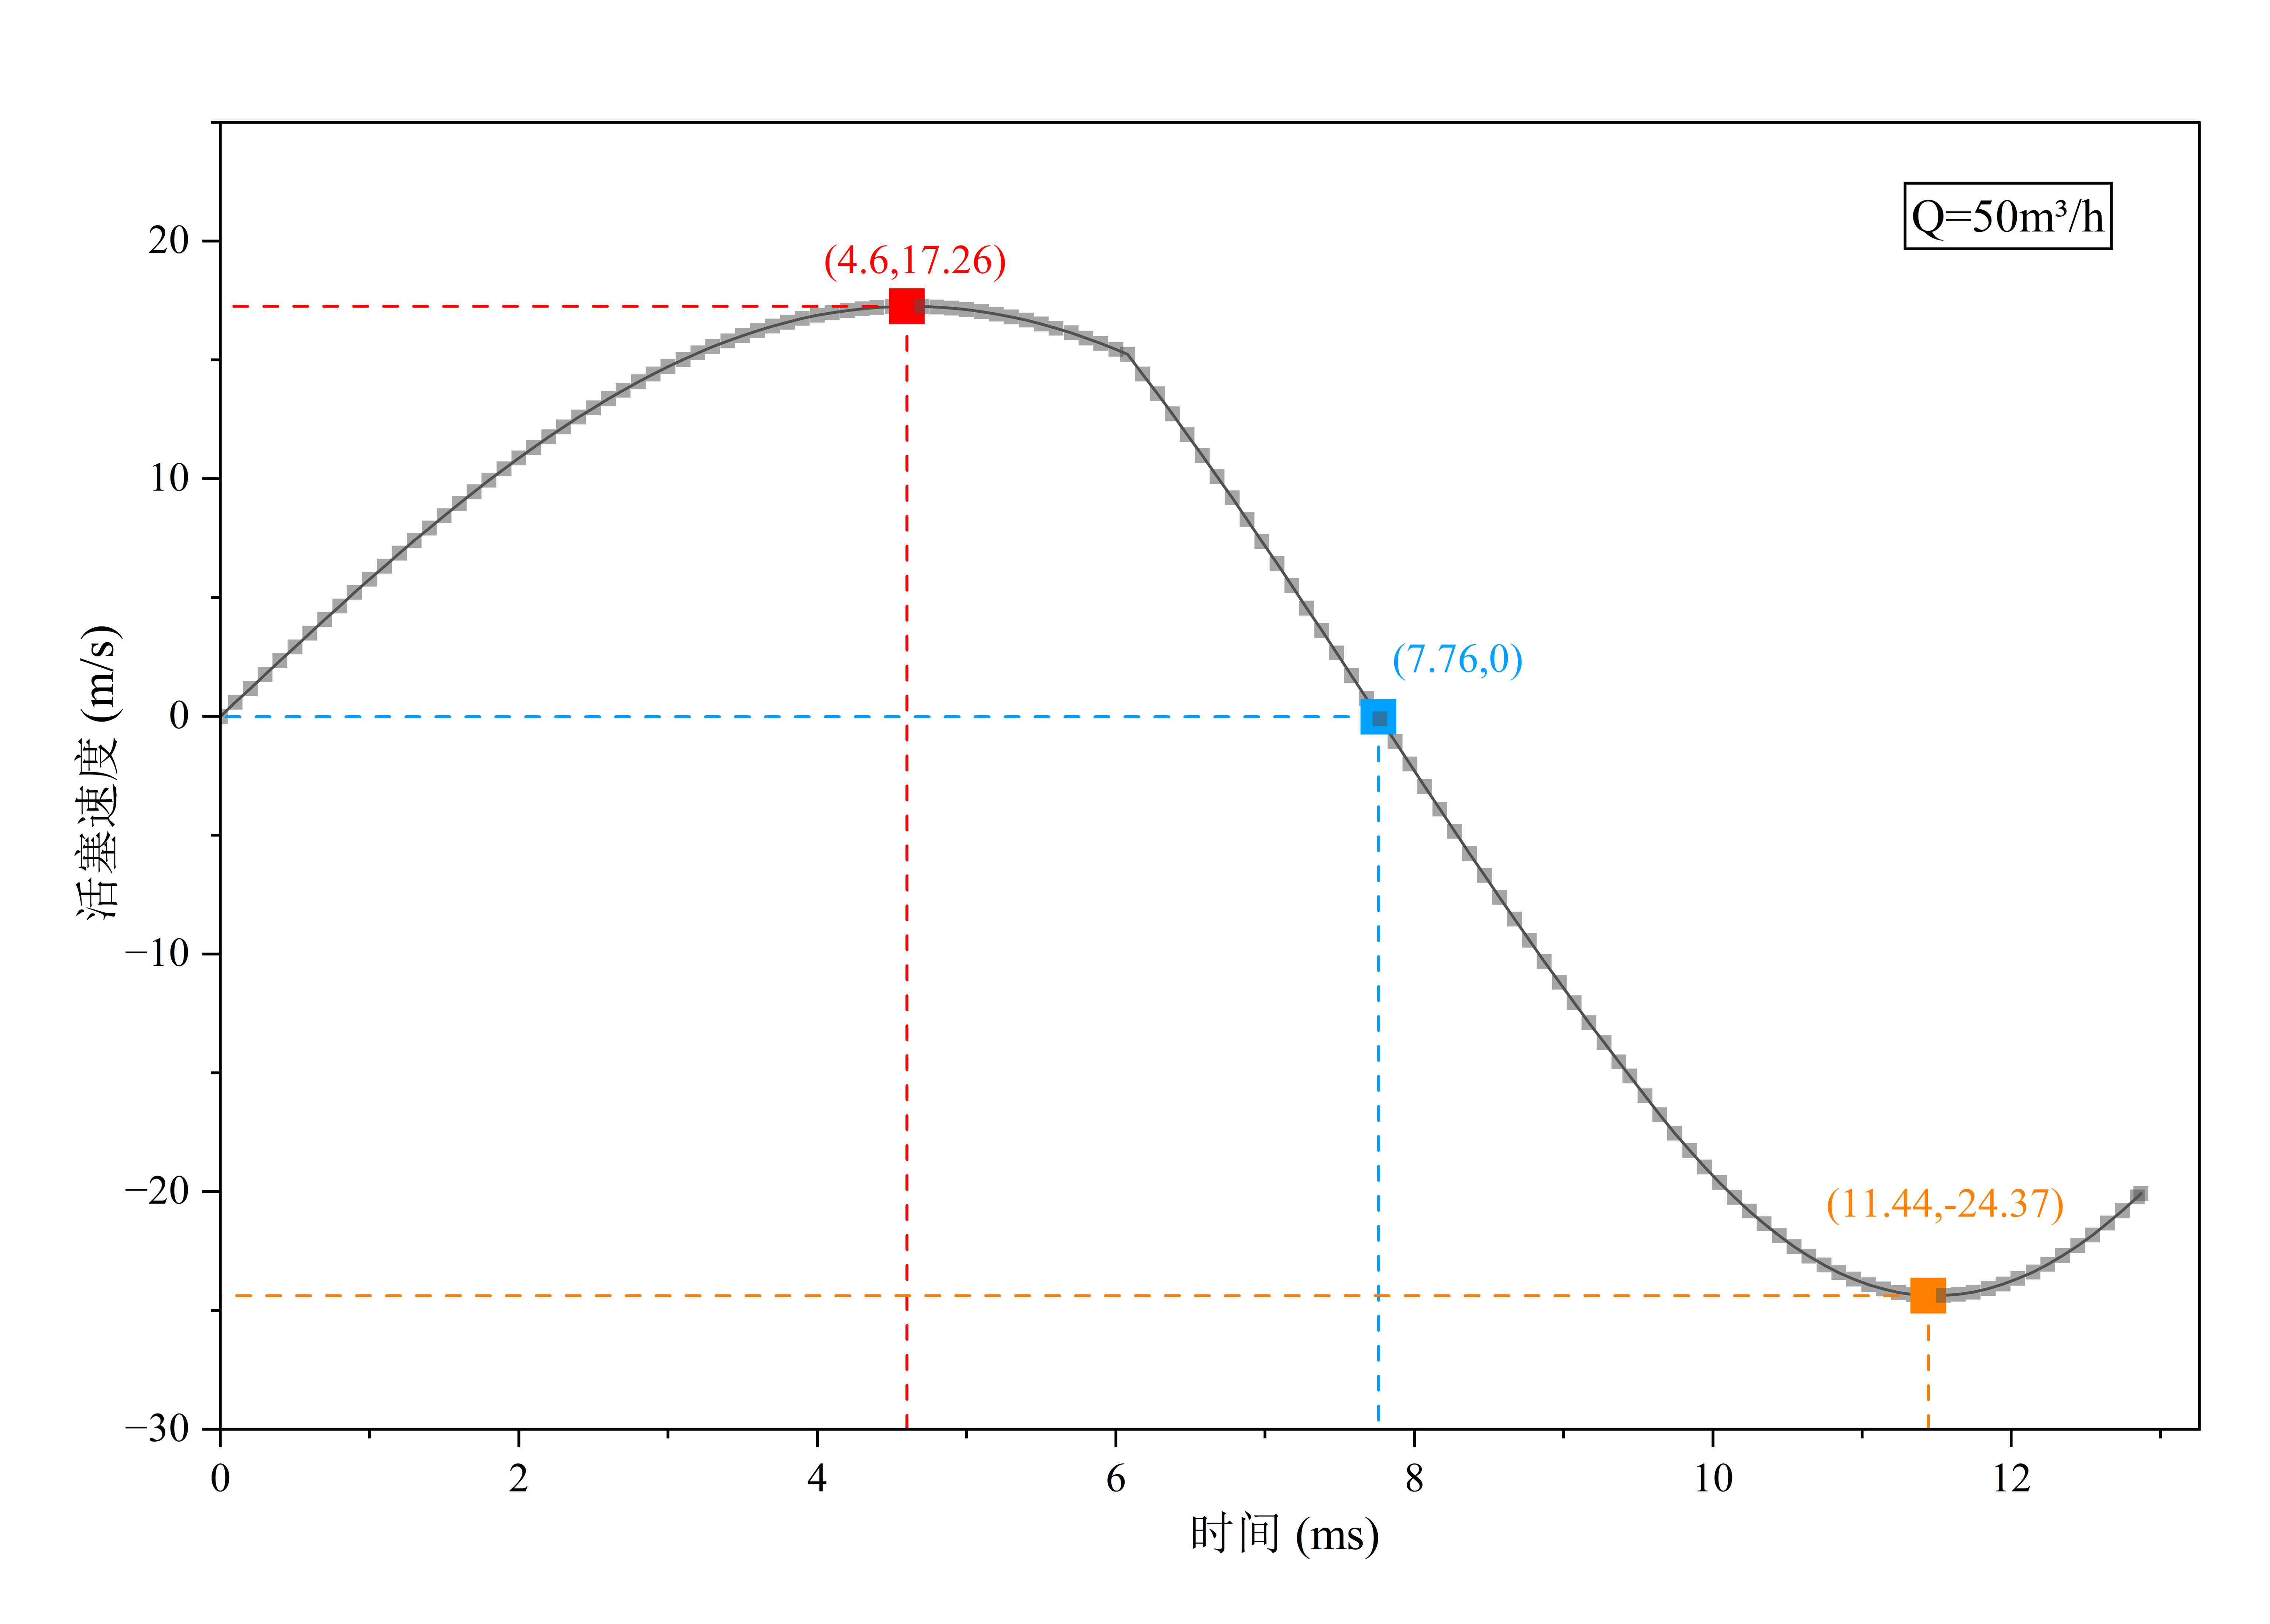
\includegraphics[width=0.7\textwidth]{figure/chapter3/piston-velocity-VS-time.png}
	\caption{活塞速度随时间变化曲线}
	\label{fig:piston_velocity_VS_time}
\end{figure}


（1）排量对脉冲发生模块频率的影响

排量$Q$是脉冲发生模块作业的关键参数，为揭示输入流量对系统动态特性的影响规律，本节在$46\mathrm{m^3/h}$至$58\mathrm{m^3/h}$的工作区间内，以$2\mathrm{m^3/h}$为梯度，绘制了活塞位移与速度随时间变化曲线对比图\ref{fig:piston_displacement_VS_Q}。对比发现：

随着排量$Q$增加，活塞的最大冲程呈显著的非线性单调递增趋势。从图中可以看到，排量越大的曲线，其上升斜率越大，且位移越早达到侧向出水孔位置。同时，在曲线的右侧末端，排量越大的曲线越早回归零点。尽管活塞位移上升阶段各曲线分离明显，但在越过峰值后的复位阶段，各组曲线下降斜率差异较小，均极其平滑地收敛于初始位置。

\begin{figure}[htbp]
	\centering
	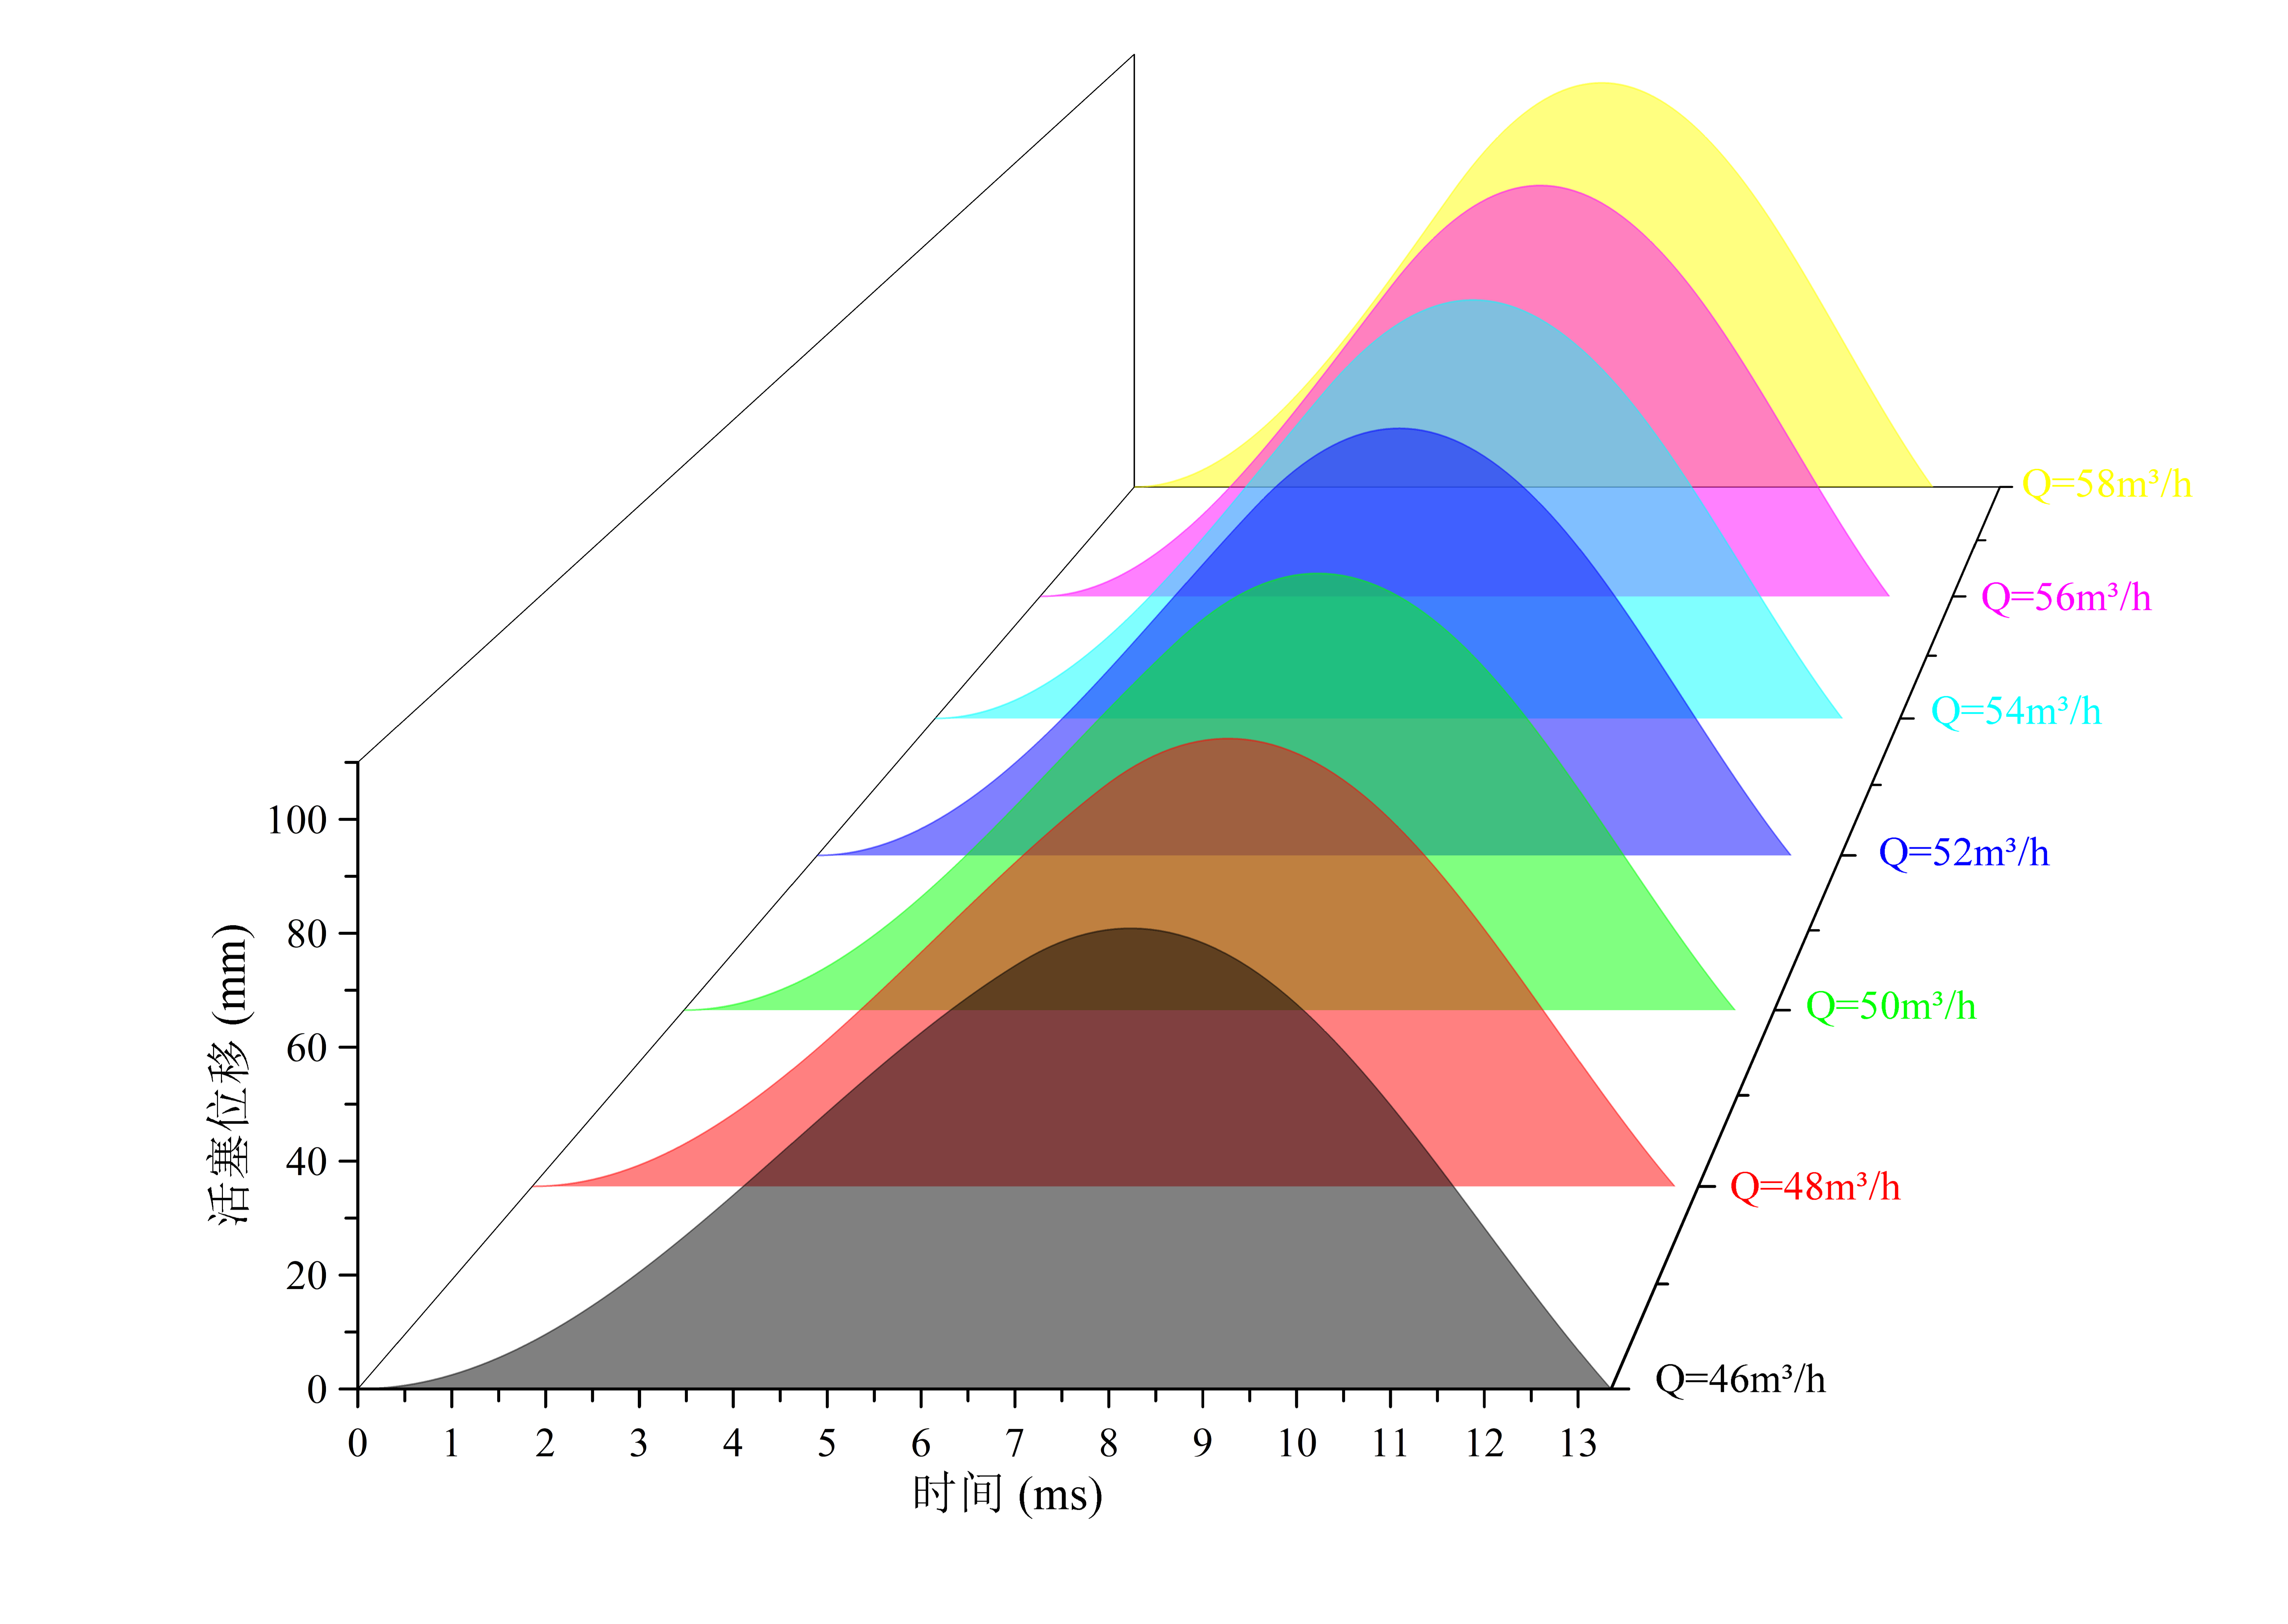
\includegraphics[width=0.7\textwidth]{figure/chapter3/piston-displacement-VS-Q.png}
	\caption{活塞位移随排量$Q$变化曲线对比图}
	\label{fig:piston_displacement_VS_Q}
\end{figure}


活塞速度随排量$Q$变化曲线如图\ref{fig:piston_velocity_VS_Q}所示，观察速度曲线的正向速度区，随着排量$Q$增加，速度曲线的波峰不仅在幅值上显著拔高（从$46m^3/h$的$14.5m/s$到$58m^3/h$的$23.1m/s$，且峰值出现的时间节点明显向左偏移。观察速度曲线的负向速度区，各排量下的弹簧回弹阶段均出现波谷。排量$Q$越大，负向速度的绝对值越大。在正向速度向负向速度过渡的速度零点，随着排量$Q$增加，曲线穿越时间轴的斜率变得越大。同时，整个速度波形的跨度沿时间轴显著缩短.

\begin{figure}[htbp]
	\centering
	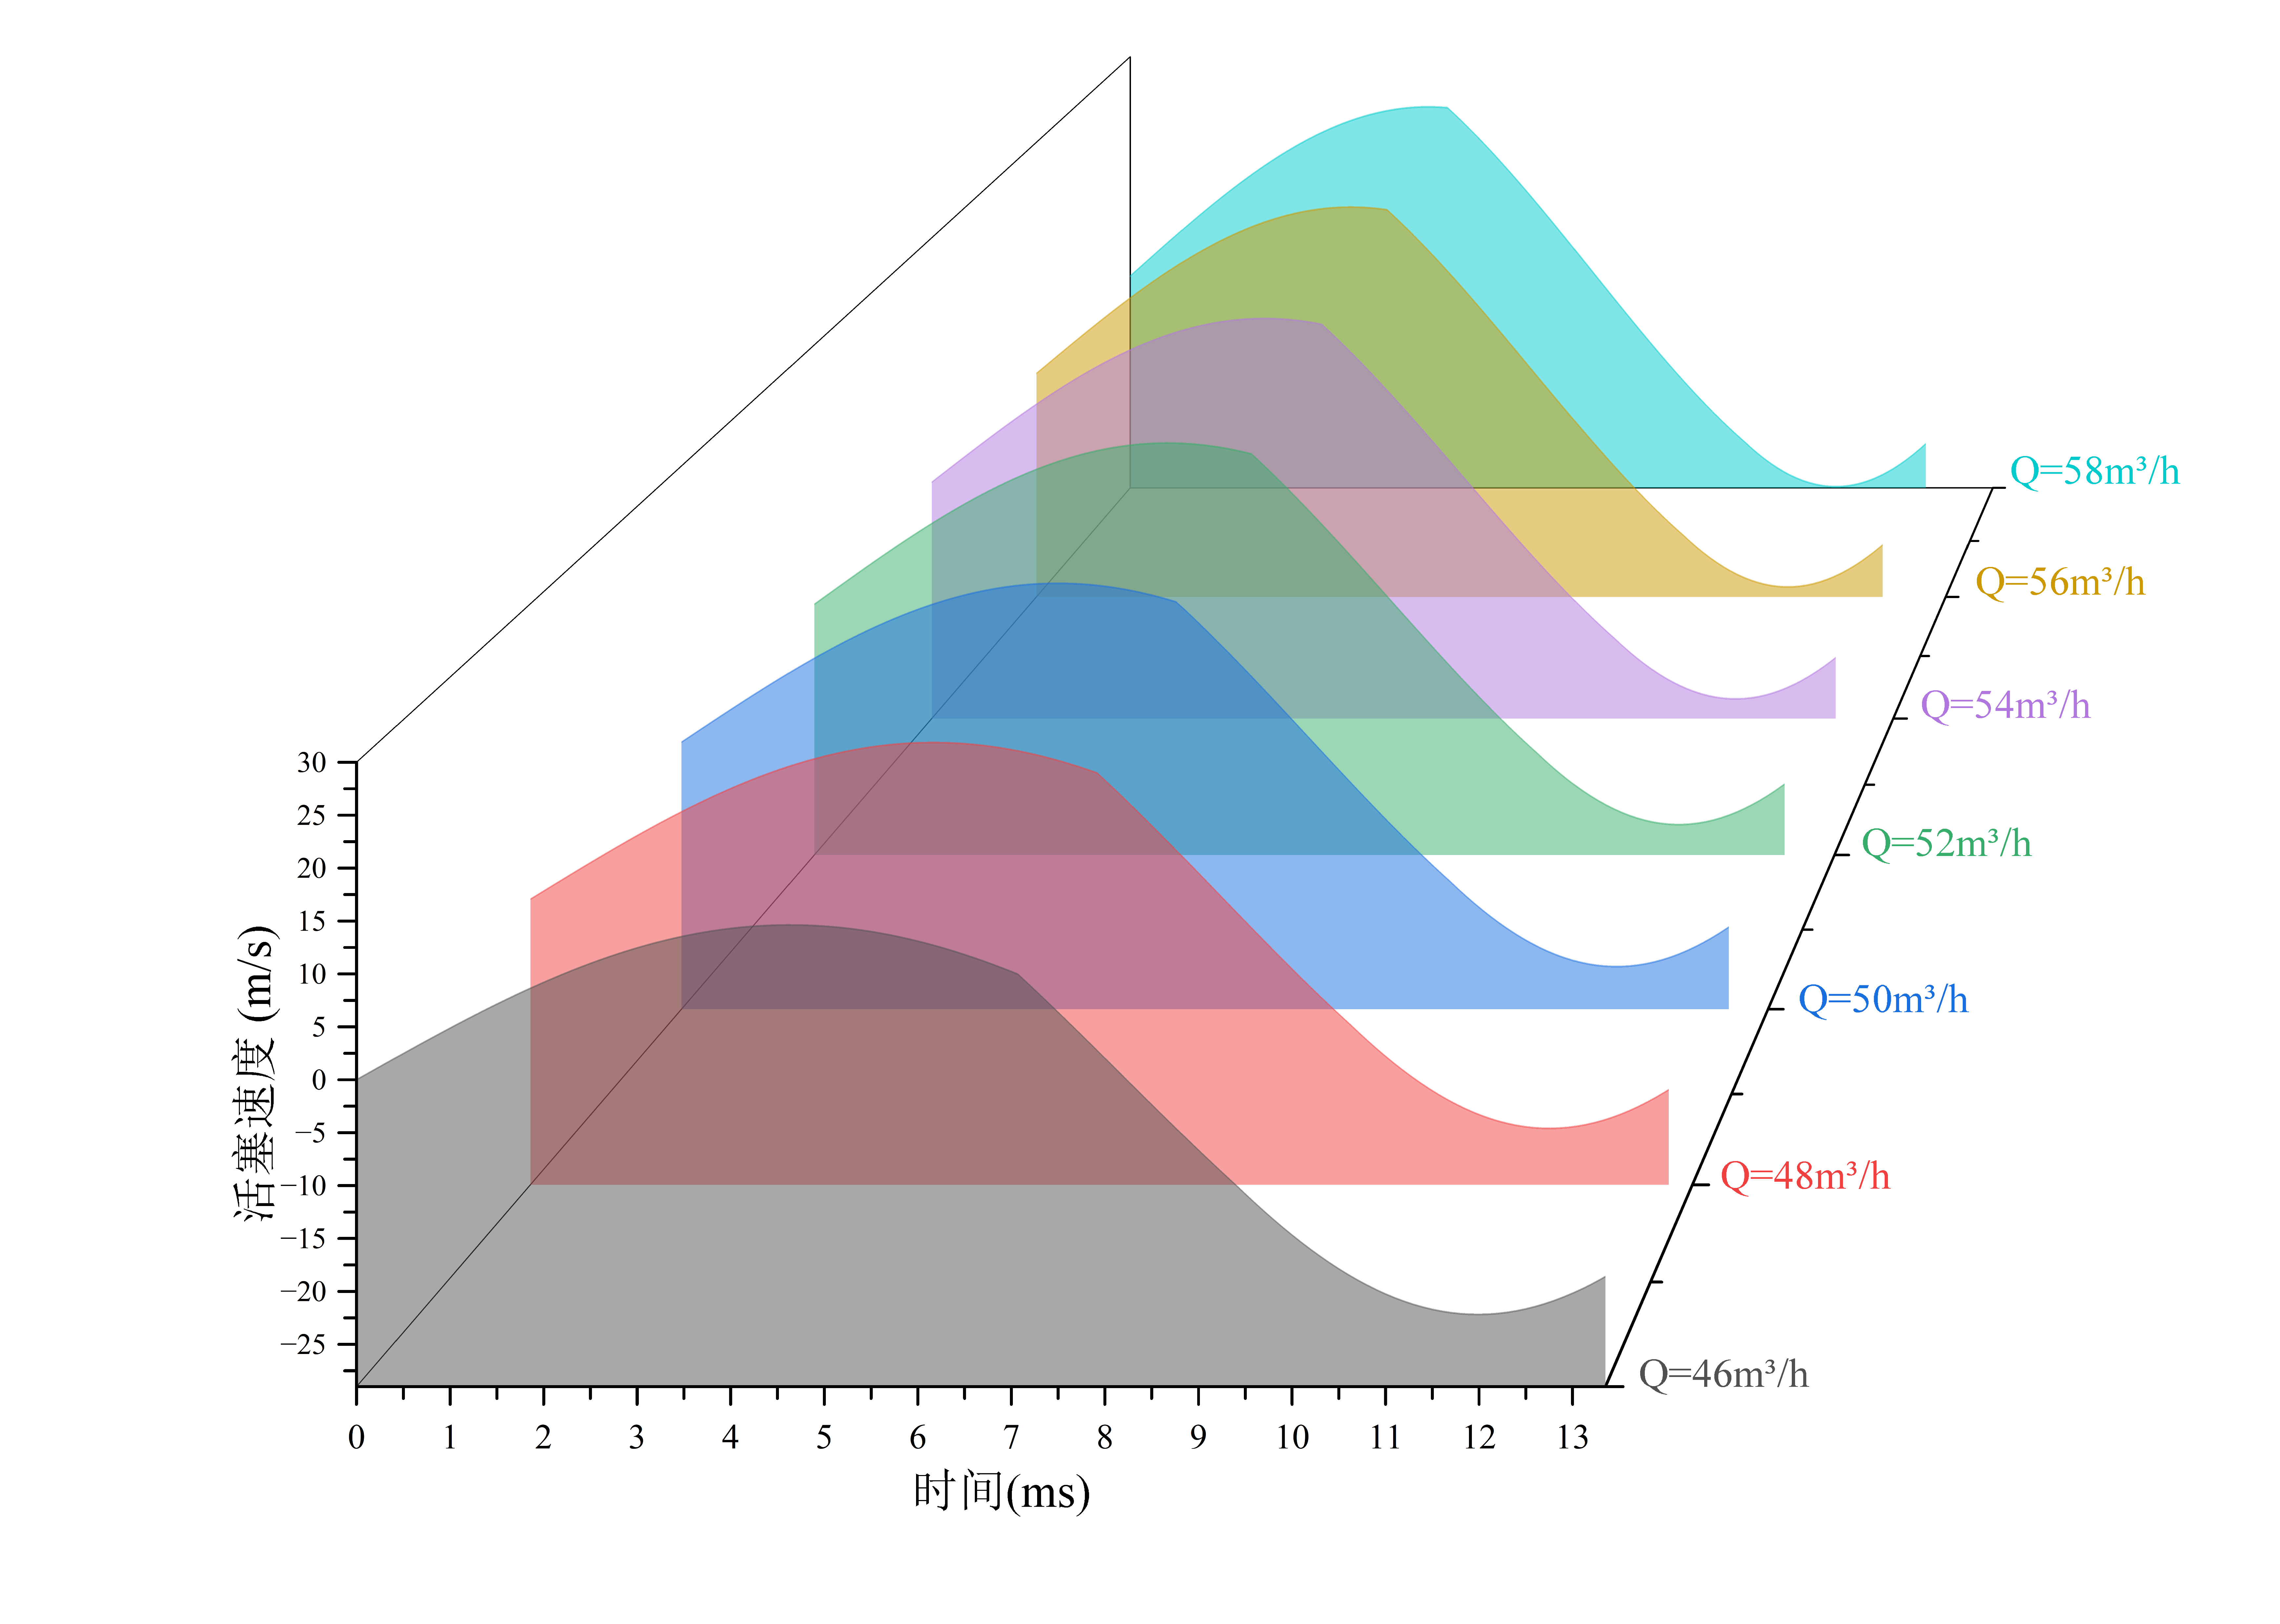
\includegraphics[width=0.7\textwidth]{figure/chapter3/piston-velocity-VS-Q.png}
	\caption{活塞速度随排量$Q$变化曲线对比图}
	\label{fig:piston_velocity_VS_Q}
\end{figure}

脉冲发生模块排量与工作频率、冲程关系特征曲线如图\ref{fig:pulse_module_frequency_stroke_VS_Q}所示，由图可知，在额定工作区间内，活塞最大冲程对流量 的变化极其敏感，且呈现出高度稳定的准线性增长趋势。提高流量能有效提升脉冲发生模块的工作频率 ，但其演化轨迹表现出明显的非线性特征。

\begin{figure}[htbp]
	\centering
	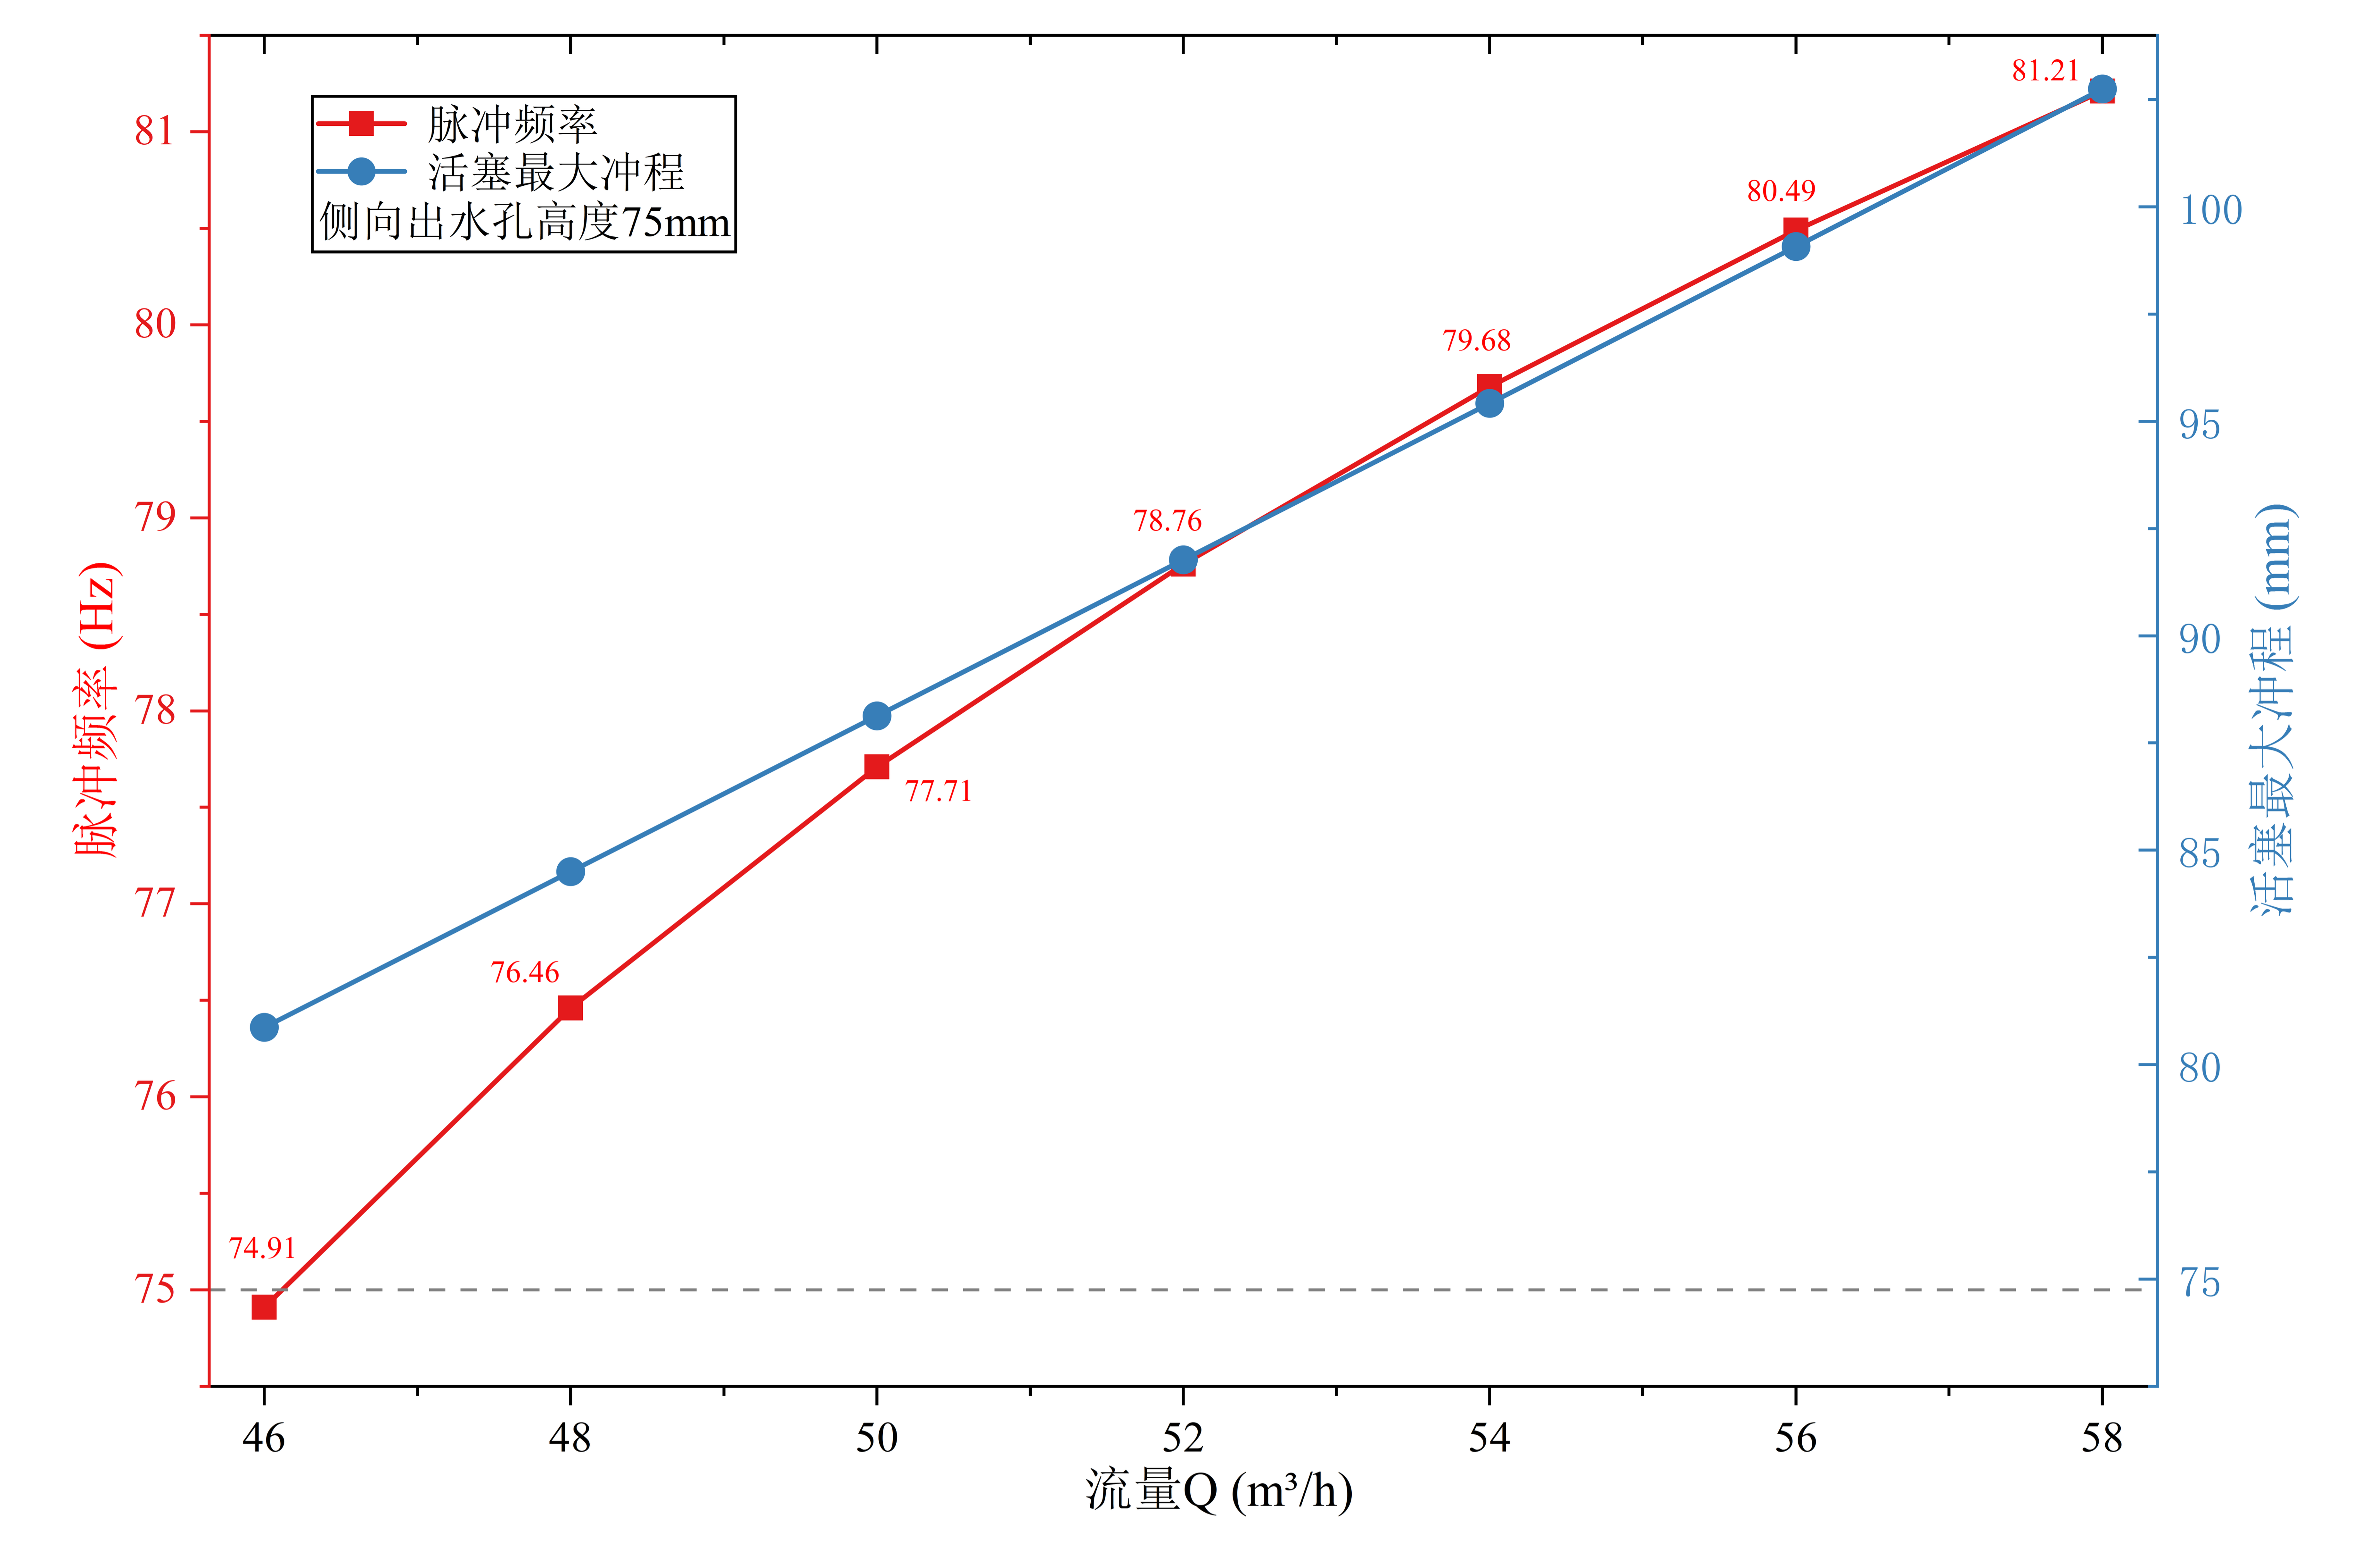
\includegraphics[width=0.7\textwidth]{figure/chapter3/pulse-module-frequency-stroke-VS-Q.png}
	\caption{脉冲发生模块排量与工作频率、冲程关系特征曲线}
	\label{fig:pulse_module_frequency_stroke_VS_Q}
\end{figure}

（2）矩形弹簧刚度对脉冲发生模块频率的影响

弹簧刚度$K$是脉冲发生模块结构设计的关键参数，为揭示弹簧刚度$K$对系统动态特性的影响规律，本节在$K=557176N/m$至$857176N/m$的设计区间内，以$50000N/m$为梯度，绘制了活塞位移与速度随时间变化曲线对比图\ref{fig:piston_displacement_VS_spring_K}。对比发现，随着弹簧刚度$K$的逐级递增，活塞位移波峰高度呈现出明显的阶梯式下降。在输入排量$Q$保持不变的前提下，高刚度弹簧能够以更短的变形距离吸收完相同的流体动能，从而使活塞最大冲程减小。观察时间轴可以发现，活塞刚度越大，其波形越窄，且波峰到达的时间节点整体向左侧发生偏移。刚度增加使活塞复位阶段动力增大，位移下降曲线斜率增大，减少了单次循环的时间。

\begin{figure}[htbp]
	\centering
	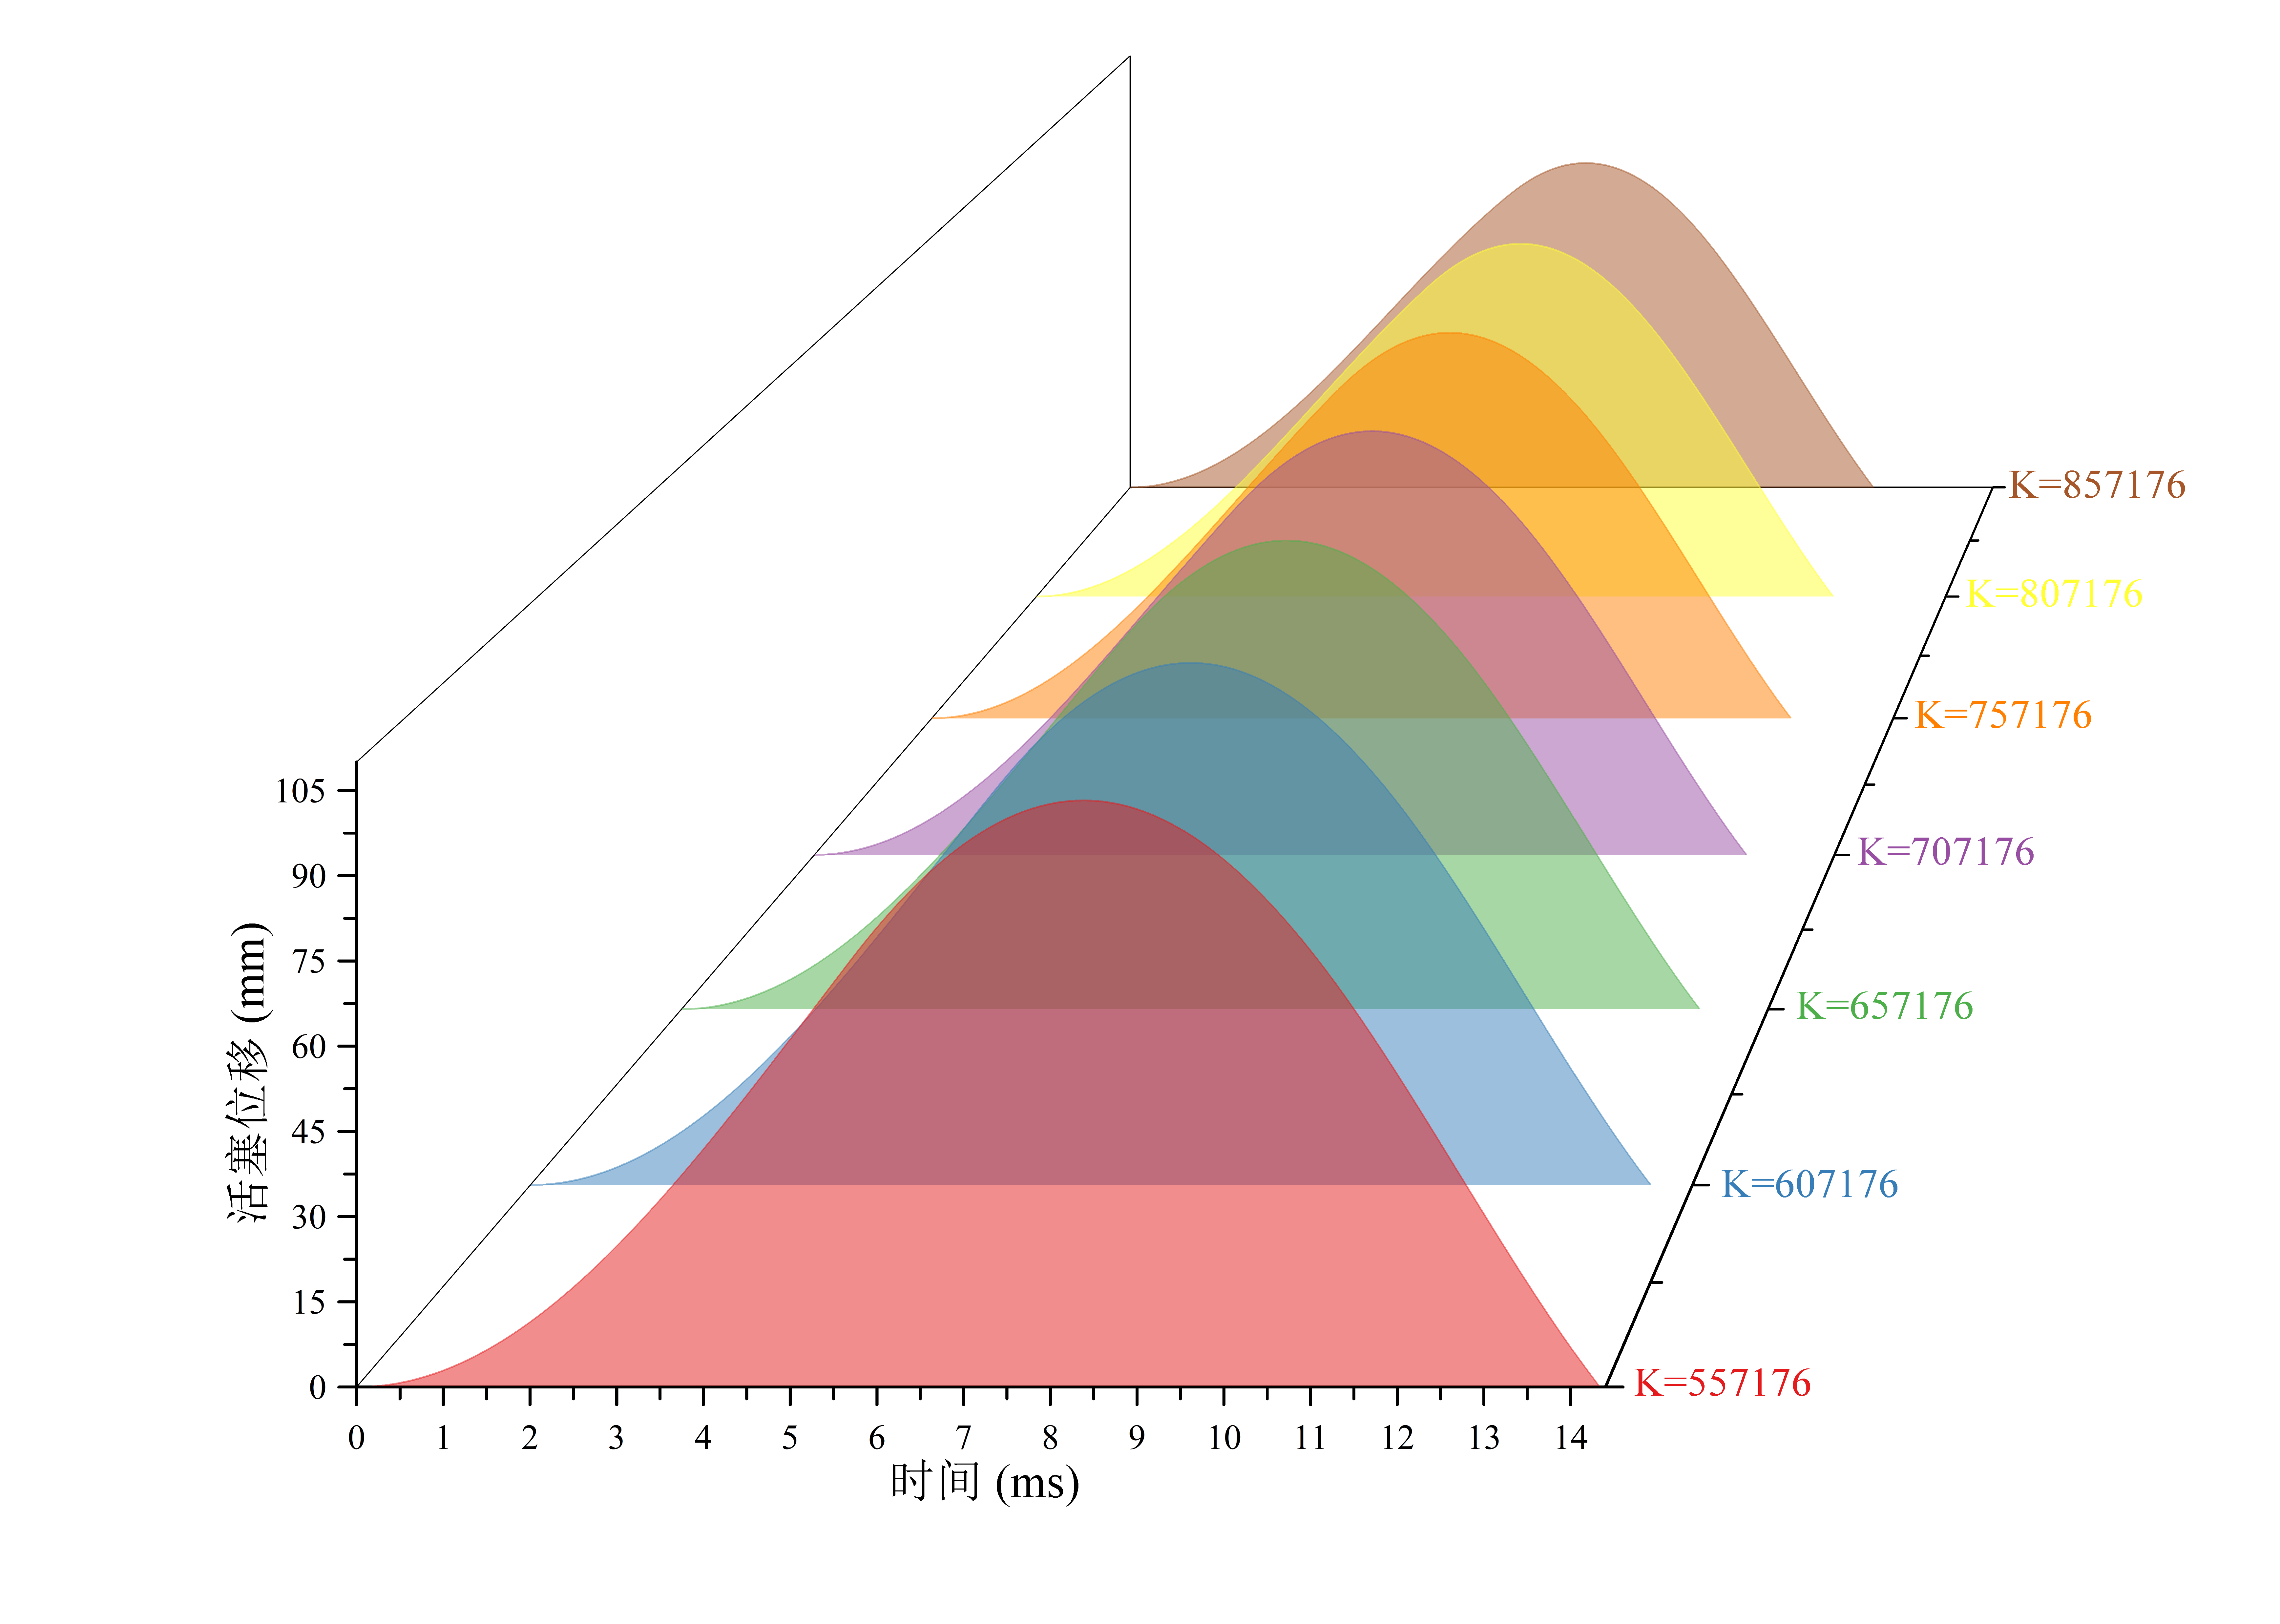
\includegraphics[width=0.7\textwidth]{figure/chapter3/piston-displacement-VS-spring-K.png}
	\caption{脉冲发生模块排量与工作频率、冲程关系特征曲线}
	\label{fig:piston_displacement_VS_spring_K}
\end{figure}

如图\ref{fig:piston_velocity_VS_spring_K}所示，随着弹簧刚度$K$的逐级递增，正向速度的波峰高度呈现阶梯式衰减，且波峰出现的时刻逐渐向左侧偏移。弹簧刚度$K$的增大使弹簧的压缩阻力增大，导致活塞正向最高速度下降，同时也使系统更早达到受力平衡点，从而表现为速度峰值的相位超前。随着弹簧刚度$K$的逐级递增，弹簧的弹性恢复力越大，活塞达到最大位移后，速度下降的斜率越大。随着弹簧刚度$K$的逐级递增，活塞的负向最高速度反而减小。尽管高刚度弹簧的初始回弹加速度更大，但由于其限制了活塞的最大冲程，导致其整体蓄积的弹性势能和可供加速的复位距离双双受限。

\begin{figure}[htbp]
	\centering
	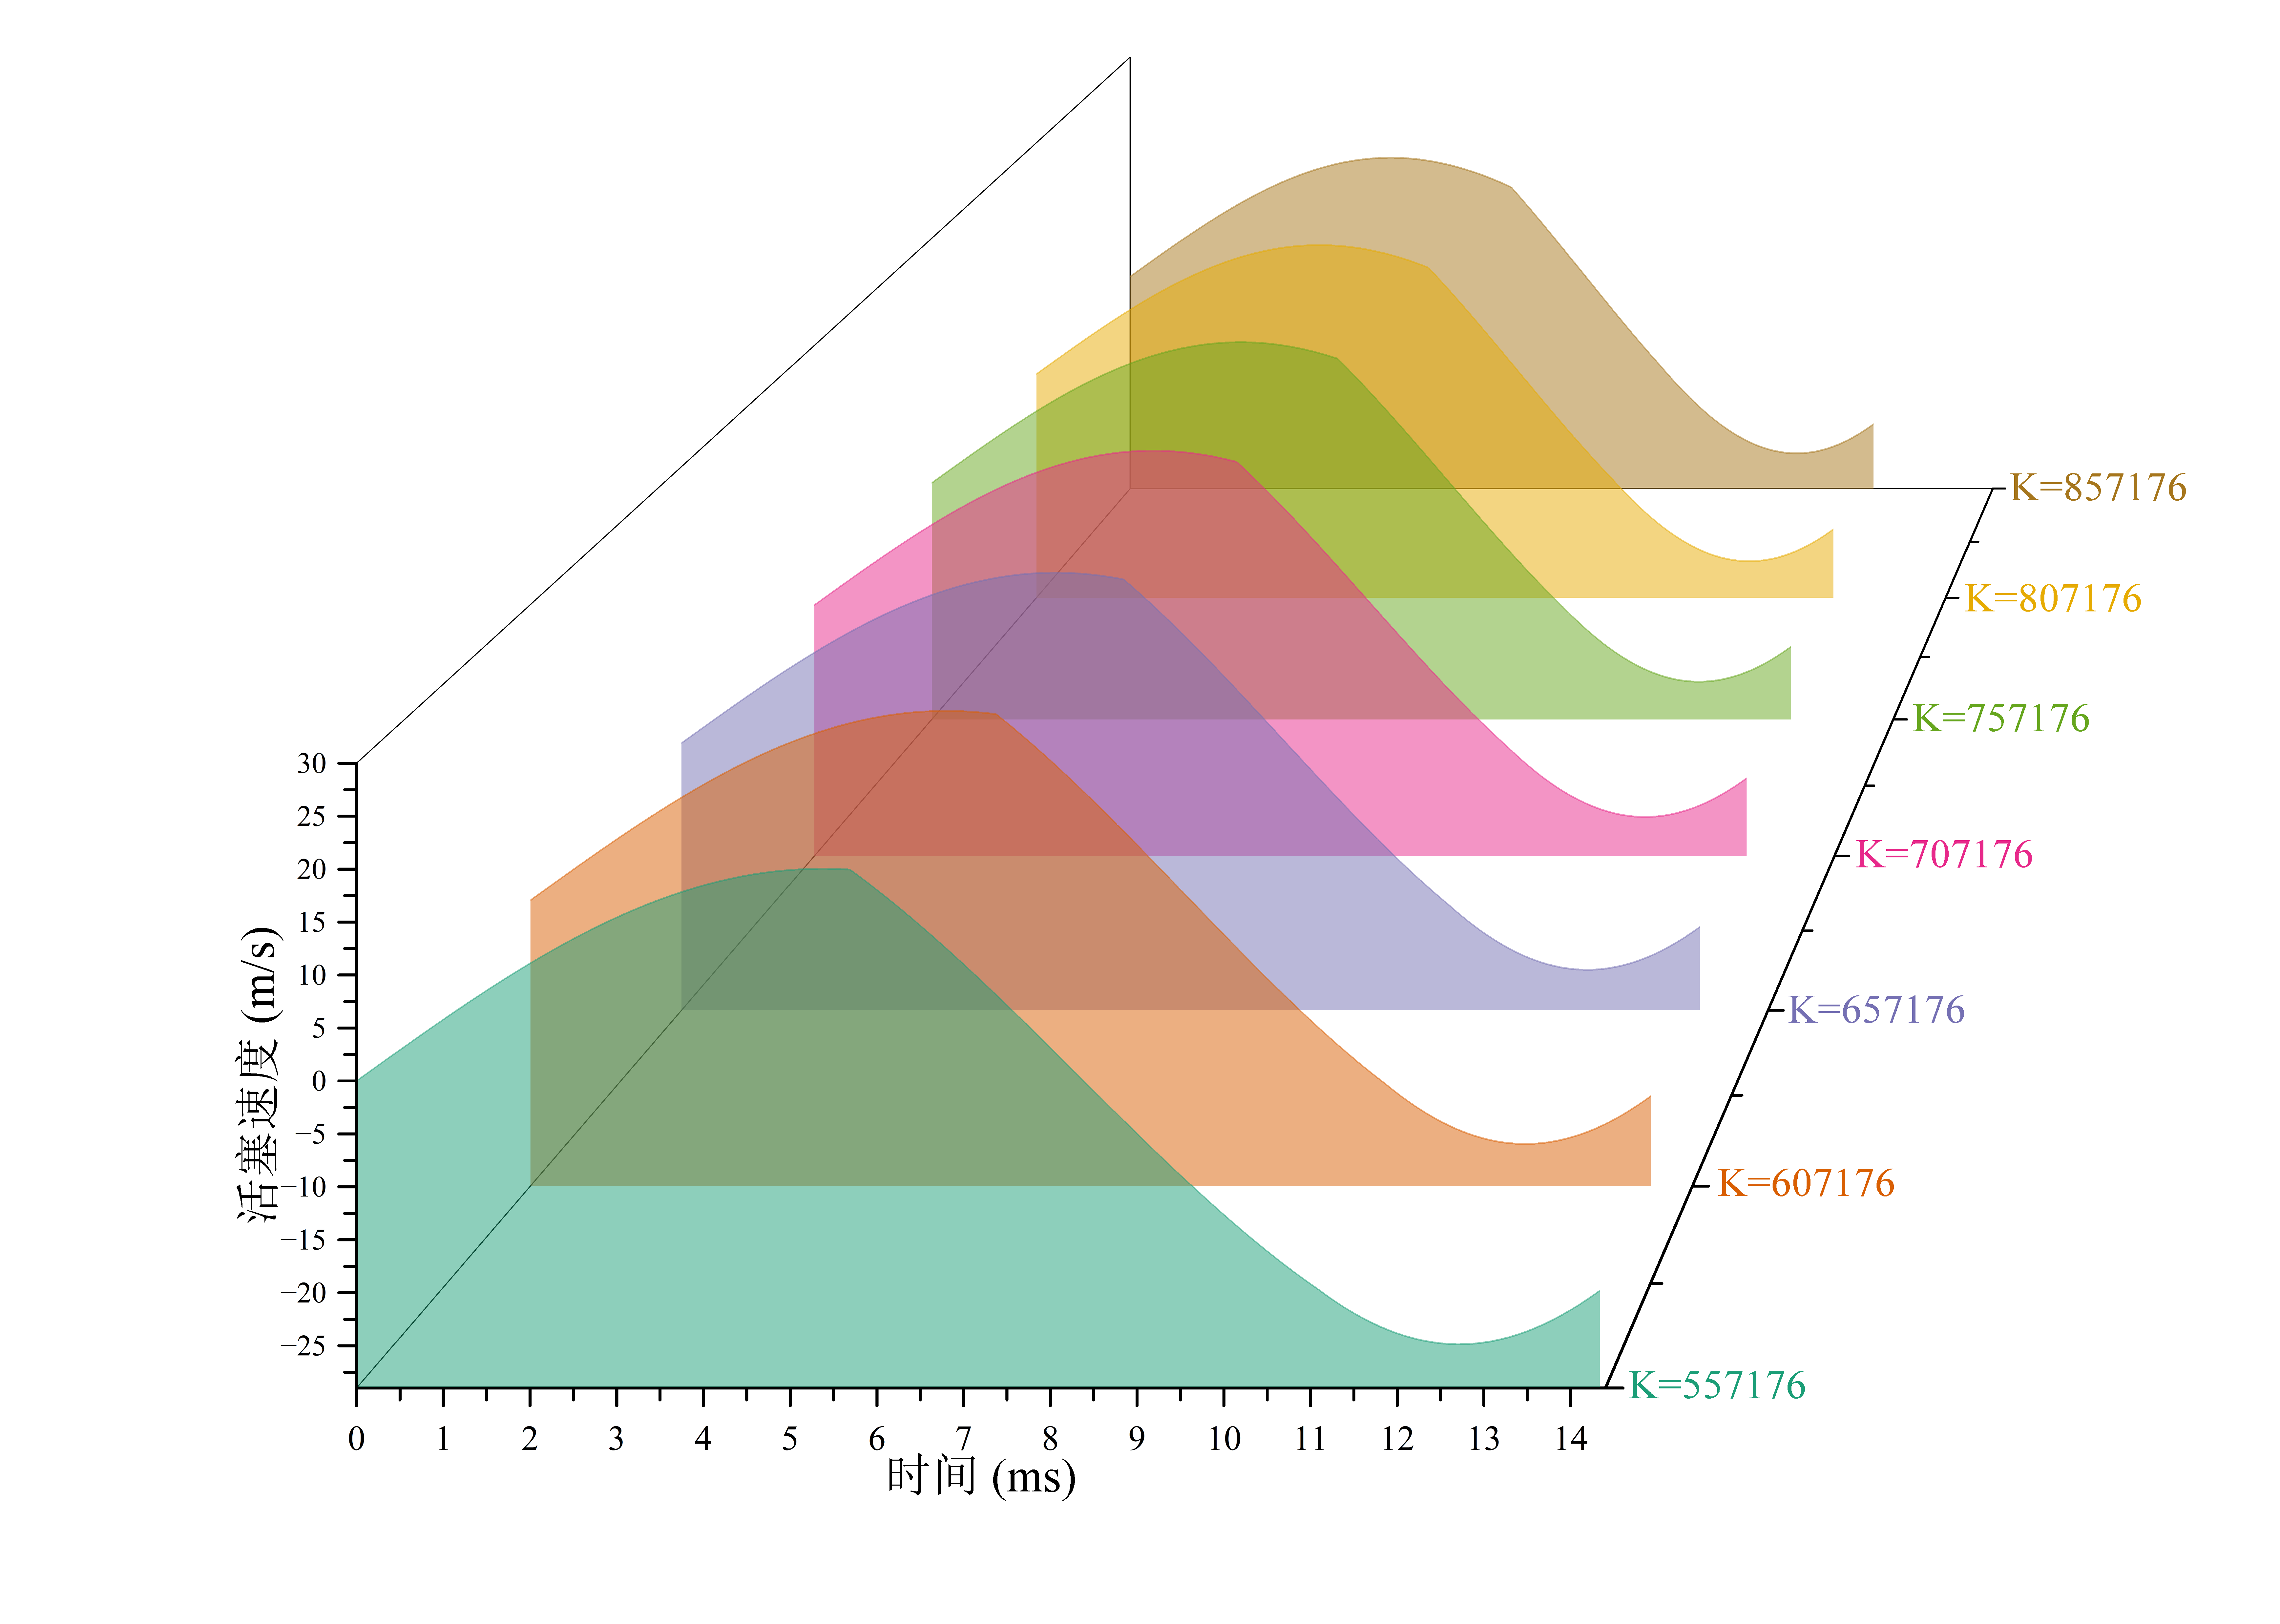
\includegraphics[width=0.7\textwidth]{figure/chapter3/piston-velocity-VS-spring-K.png}
	\caption{活塞速度随弹簧刚度$K$变化曲线对比图}
	\label{fig:piston_velocity_VS_spring_K}
\end{figure}

脉冲发生模块弹簧刚度$K$与工作频率、冲程关系特征曲线如图4.16所示，由图可知，随着弹簧刚度的逐级递增，活塞冲程呈现单调递减趋势。与冲程规律相反，工作频率随弹簧刚度的增加而增大。观察频率曲线的斜率可以发现，在低刚度向中等刚度过渡时，提频效果最为显著；但随着刚度进一步向$850kN/m$以上逼近，曲线爬升趋势放缓。这表明单纯依靠增加机械刚度来提频存在物理极限，过度强化刚度会反向制约下击效率。

\begin{figure}[htbp]
	\centering
	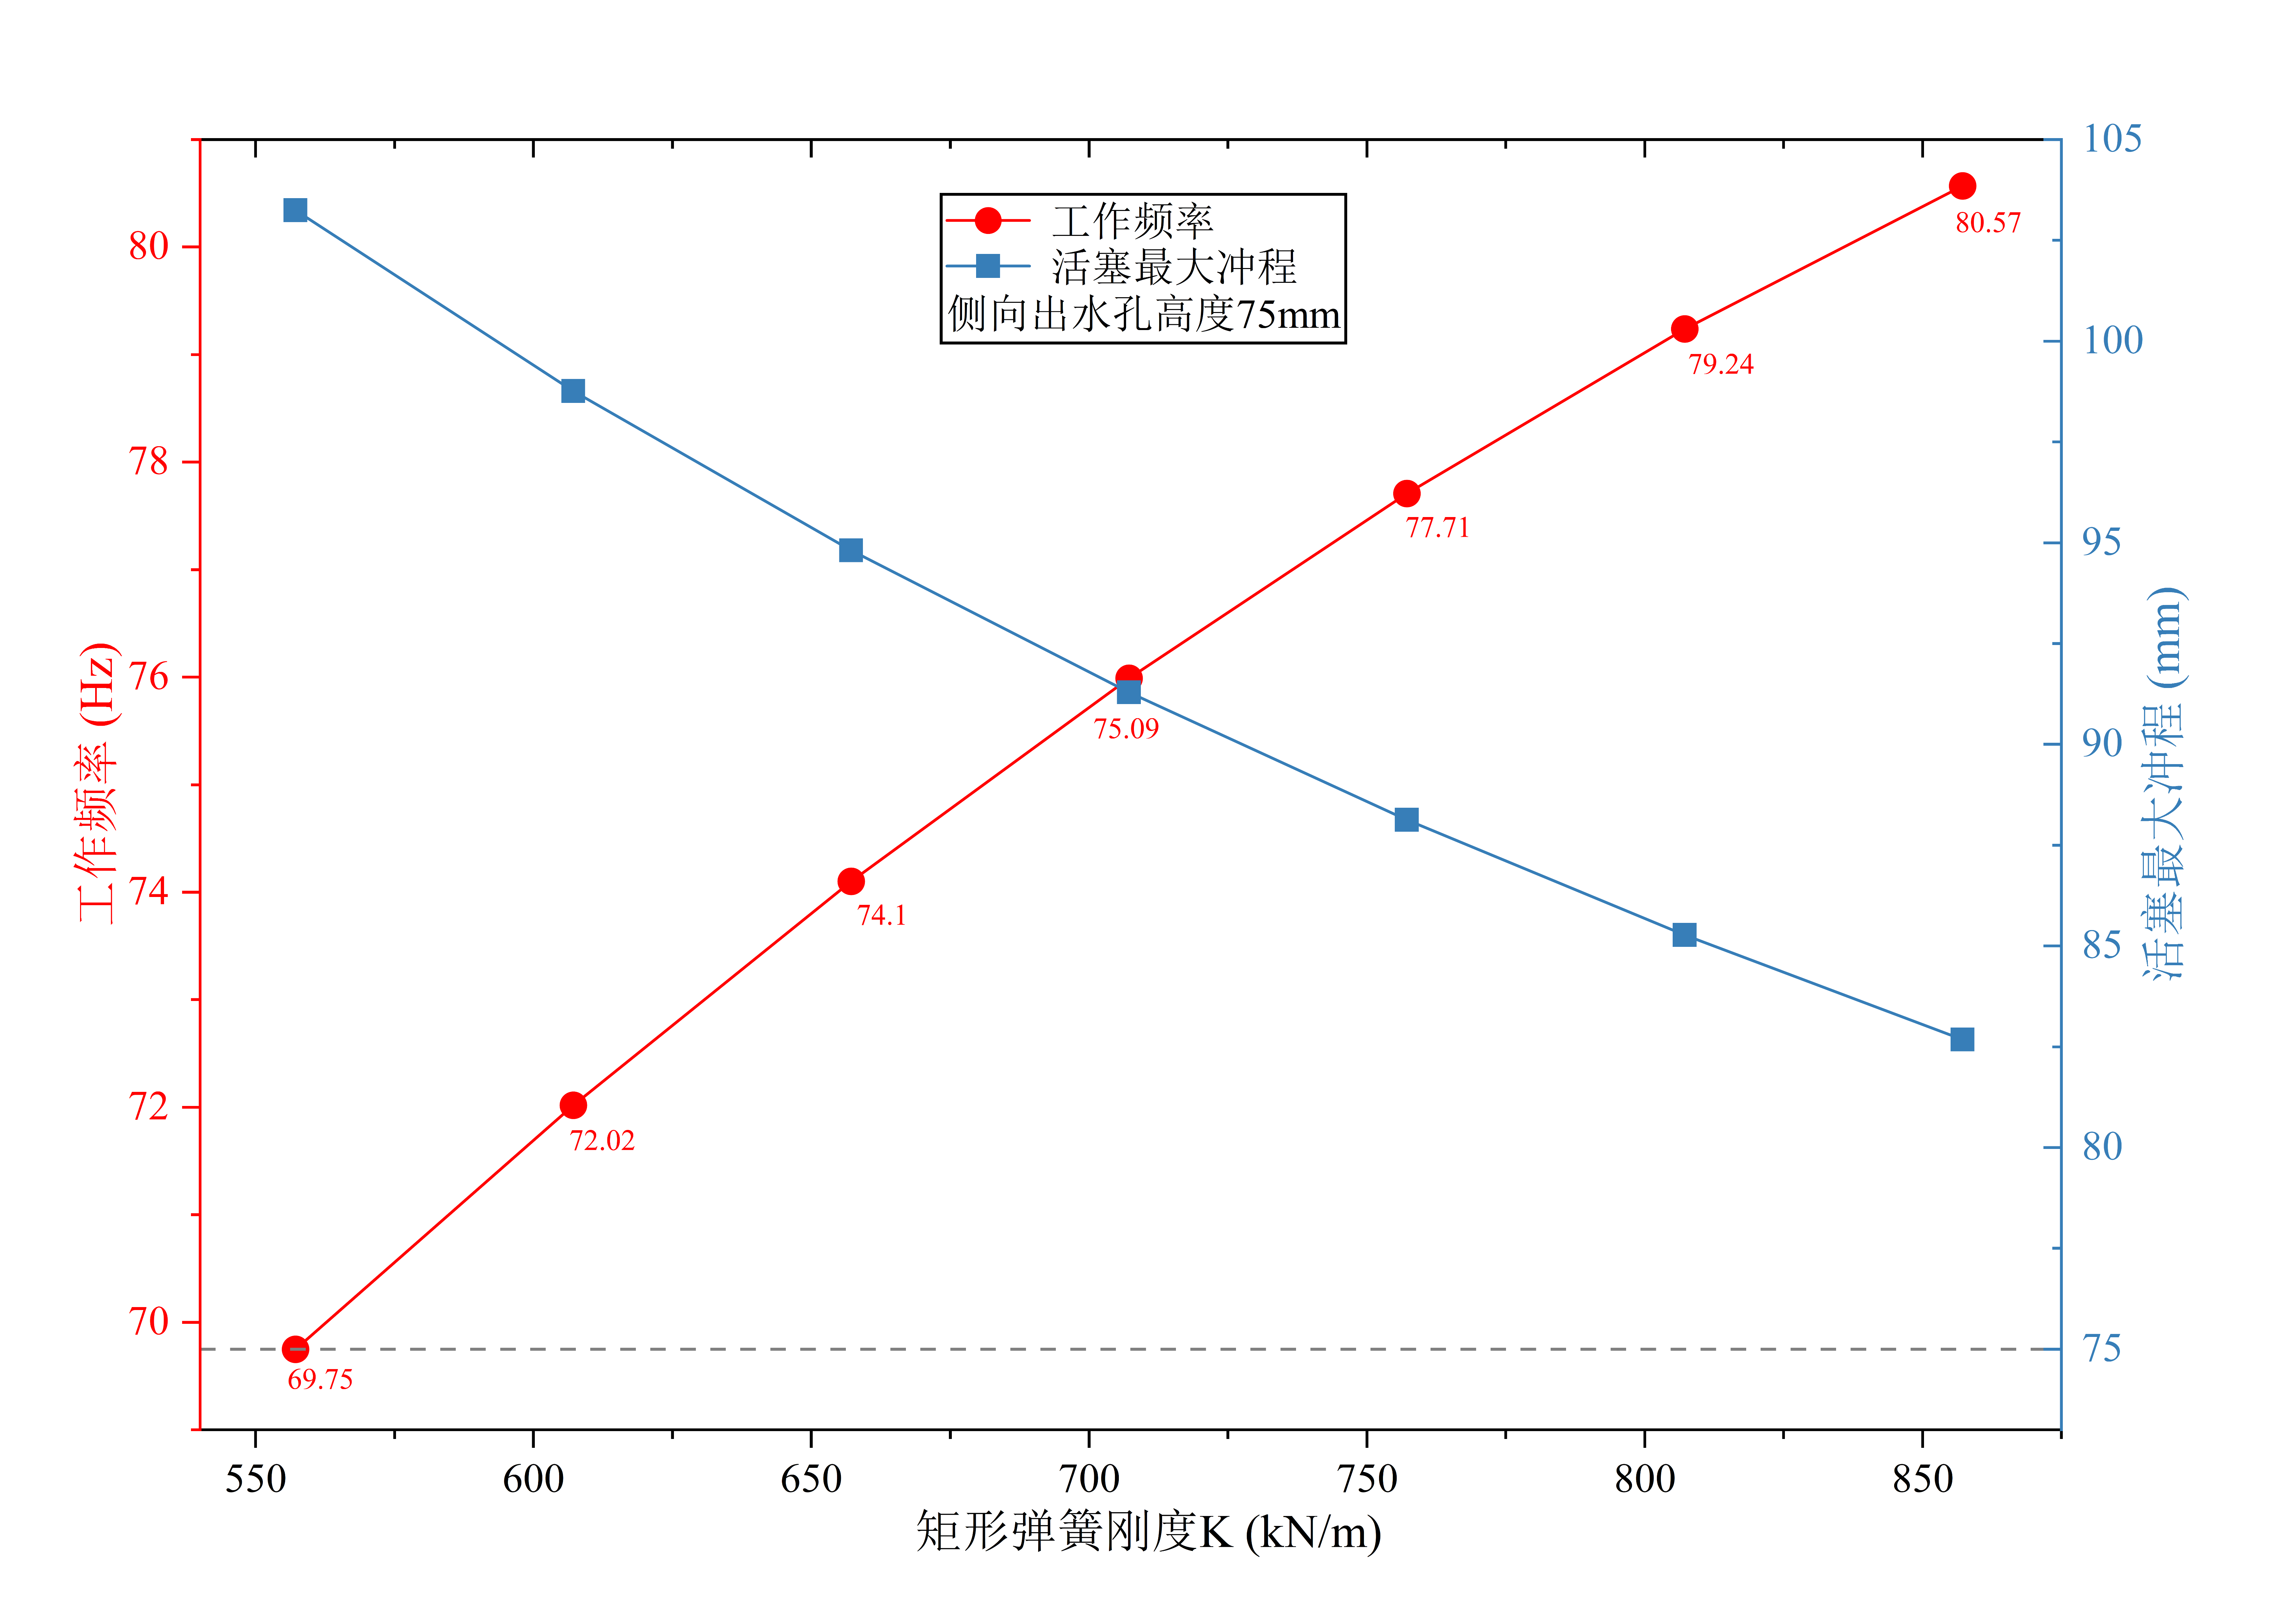
\includegraphics[width=0.7\textwidth]{figure/chapter3/pulse-module-frequency-stroke-VS-spring-K.png}
	\caption{脉冲发生模块弹簧刚度$K$与工作频率、冲程关系特征曲线}
	\label{fig:pulse_module_frequency_stroke_VS_spring_K}
\end{figure}

（3）侧向出水孔高度对脉冲发生模块频率的影响

侧向出水孔高度$h$是脉冲发生模块结构设计的关键参数，为揭示侧向出水孔高度 对系统动态特性的影响规律，本节在$h=65mm$至$90mm$的设计区间内，以$5mm$为梯度，绘制了活塞位移与速度随时间变化曲线对比图\ref{fig:piston_displacement_VS_h}。对比发现，随着$h$值的增大，活塞位移图像的波峰也随之升高，$h$值的增大也推迟了活塞越过侧向出水孔的时刻，使得蓄能阶段在整个周期中的占比增加。侧向出水孔下移不仅拉长了活塞到达最大冲程所需的时间，更因为冲程的加深，迫使活塞在复位时必须跨越更长的距离，因此活塞运动周期加长。如图\ref{fig:piston_velocity_VS_h}所示，随着$h$值的增大，活塞正向速度峰值变化不明显，这表明系统向下的综合加速度在位移小于$65mm$时便已归零并发生反转。因此，无论泄流孔是在$65mm$还是$90mm$处打开，活塞都已经提前达到正向最大速度。随着$h$值的增大，活塞正向速度波形变宽，代表着活塞维持在向下冲击状态的时间被拉长。观察活塞负向速度，随着$h$值的增大，活塞复位阶段的绝对负向速度越大。

\begin{figure}[htbp]
	\centering
	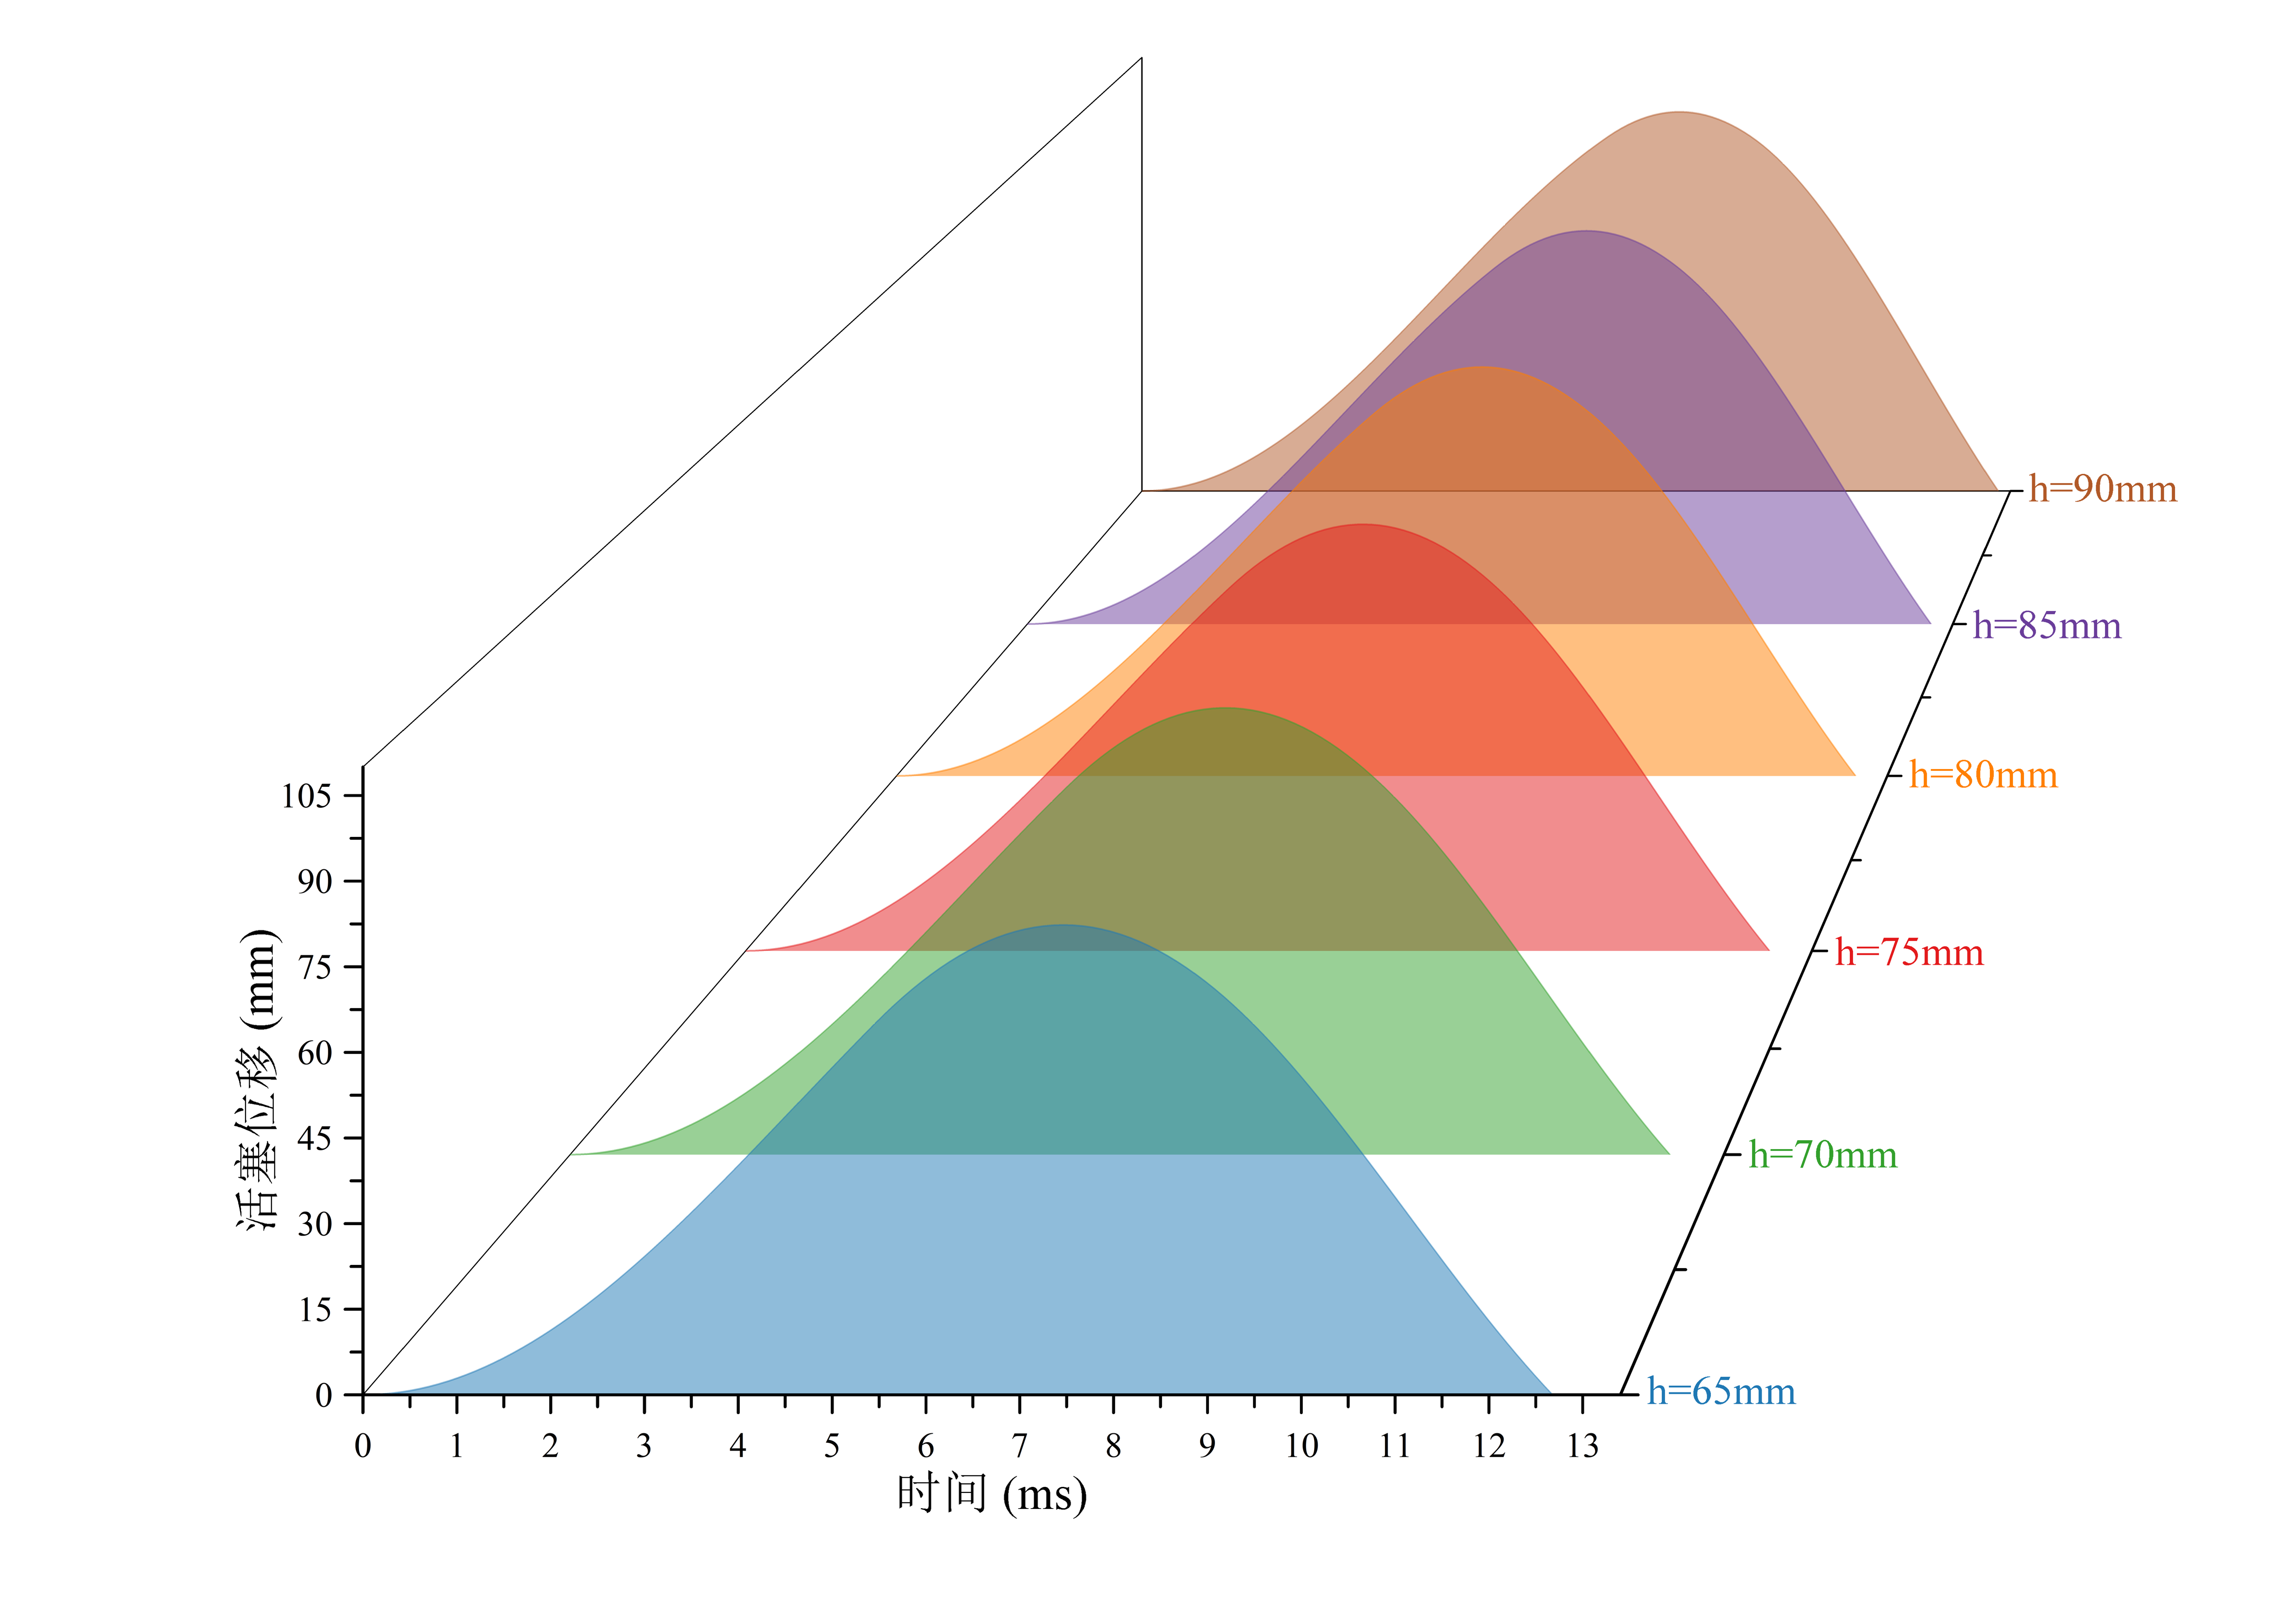
\includegraphics[width=0.7\textwidth]{figure/chapter3/piston-displacement-VS-h.png}
	\caption{活塞位移随侧向出水孔高度$h$变化曲线对比图}
	\label{fig:piston_displacement_VS_h}
\end{figure}

\begin{figure}[htbp]
	\centering
	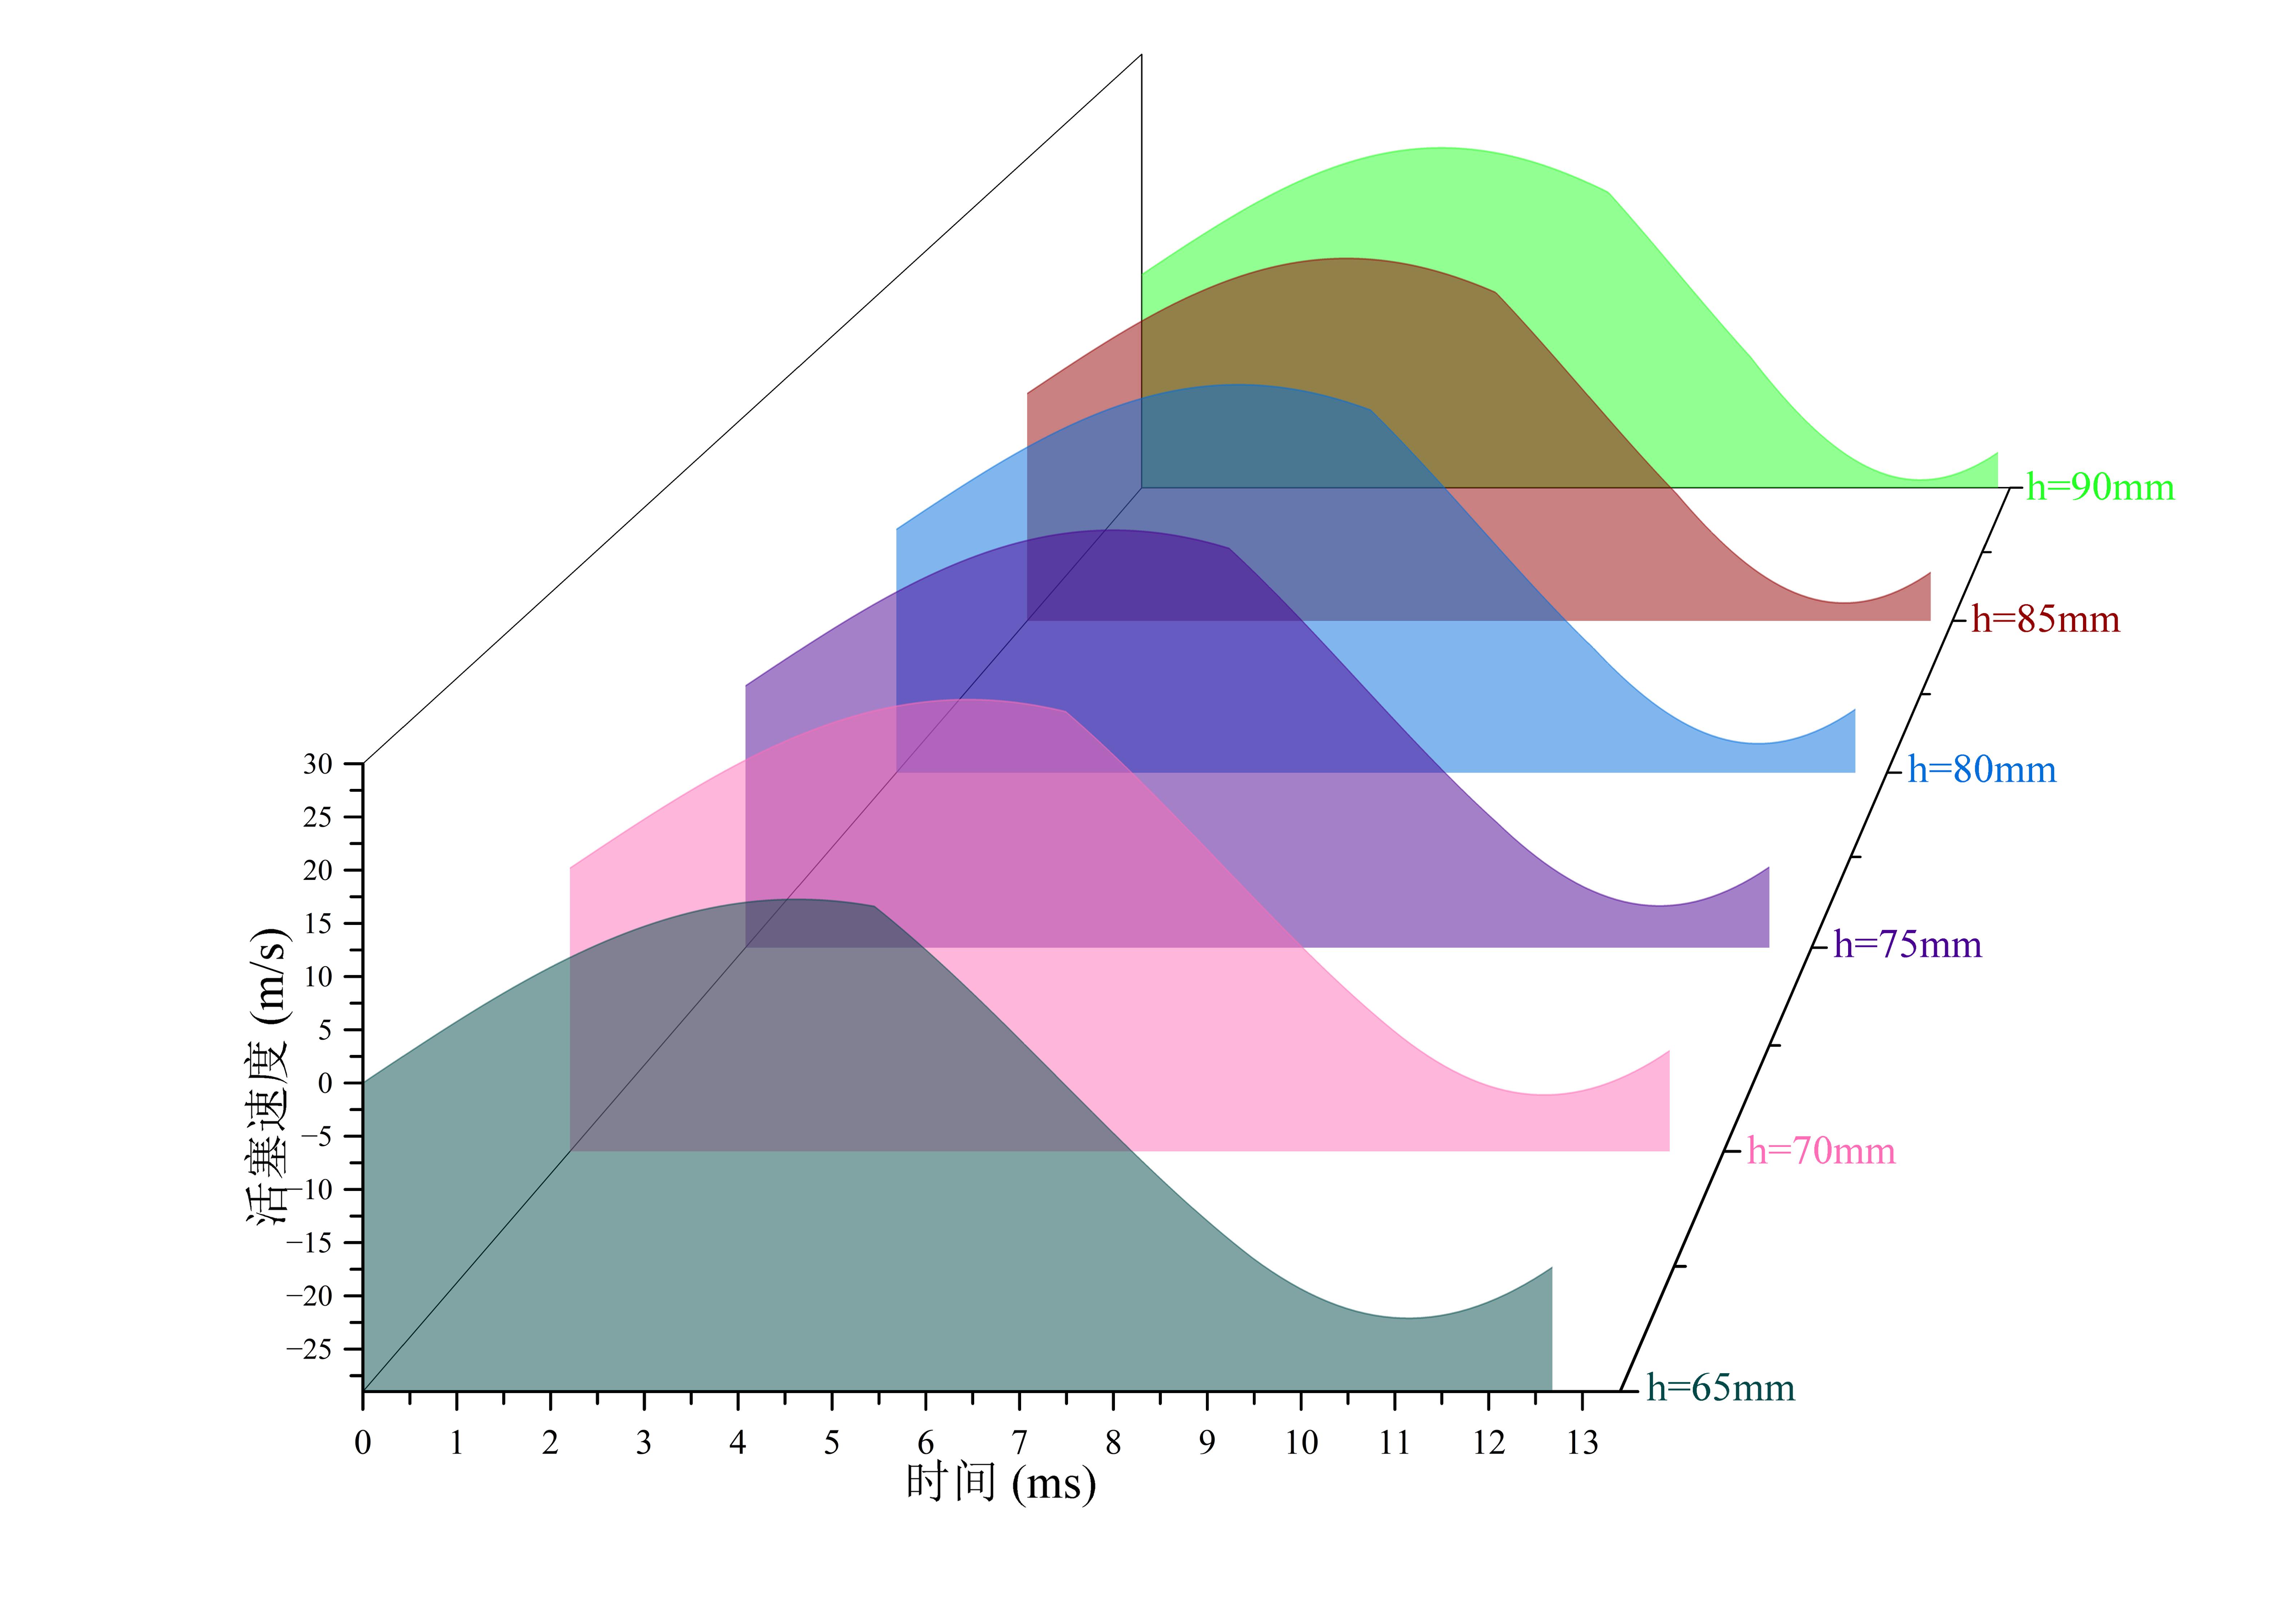
\includegraphics[width=0.7\textwidth]{figure/chapter3/piston-velocity-VS-h.png}
	\caption{活塞位移随侧向出水孔高度$h$变化曲线对比图}
	\label{fig:piston_velocity_VS_h}
\end{figure}


侧向出水孔高度对工作频率与冲程的影响特征曲线如图\ref{fig:piston_frequency_stroke_VS_h}所示，随着侧向出水孔高度$h$增大，活塞蓄能阶段距离延长，单次脉冲耗时拉长，脉冲发生模块工作频率减小。图中灰色虚点线代表了泄流孔的物理开启阈值，而蓝色实线代表活塞的最大位移距离。两者之间填充的浅蓝色阴影区域，即表征了活塞越过开孔位置后的开孔有效余量。随着侧向出水孔高度$h$增大，阴影区域的形态收缩，脉冲发生模块开孔有效余量减少，因此在设计脉冲发生模块时，应保证适宜的开孔有效余量，既要保证足够的脉冲频率，也要满足足够的活塞冲程。

\begin{figure}[htbp]
	\centering
	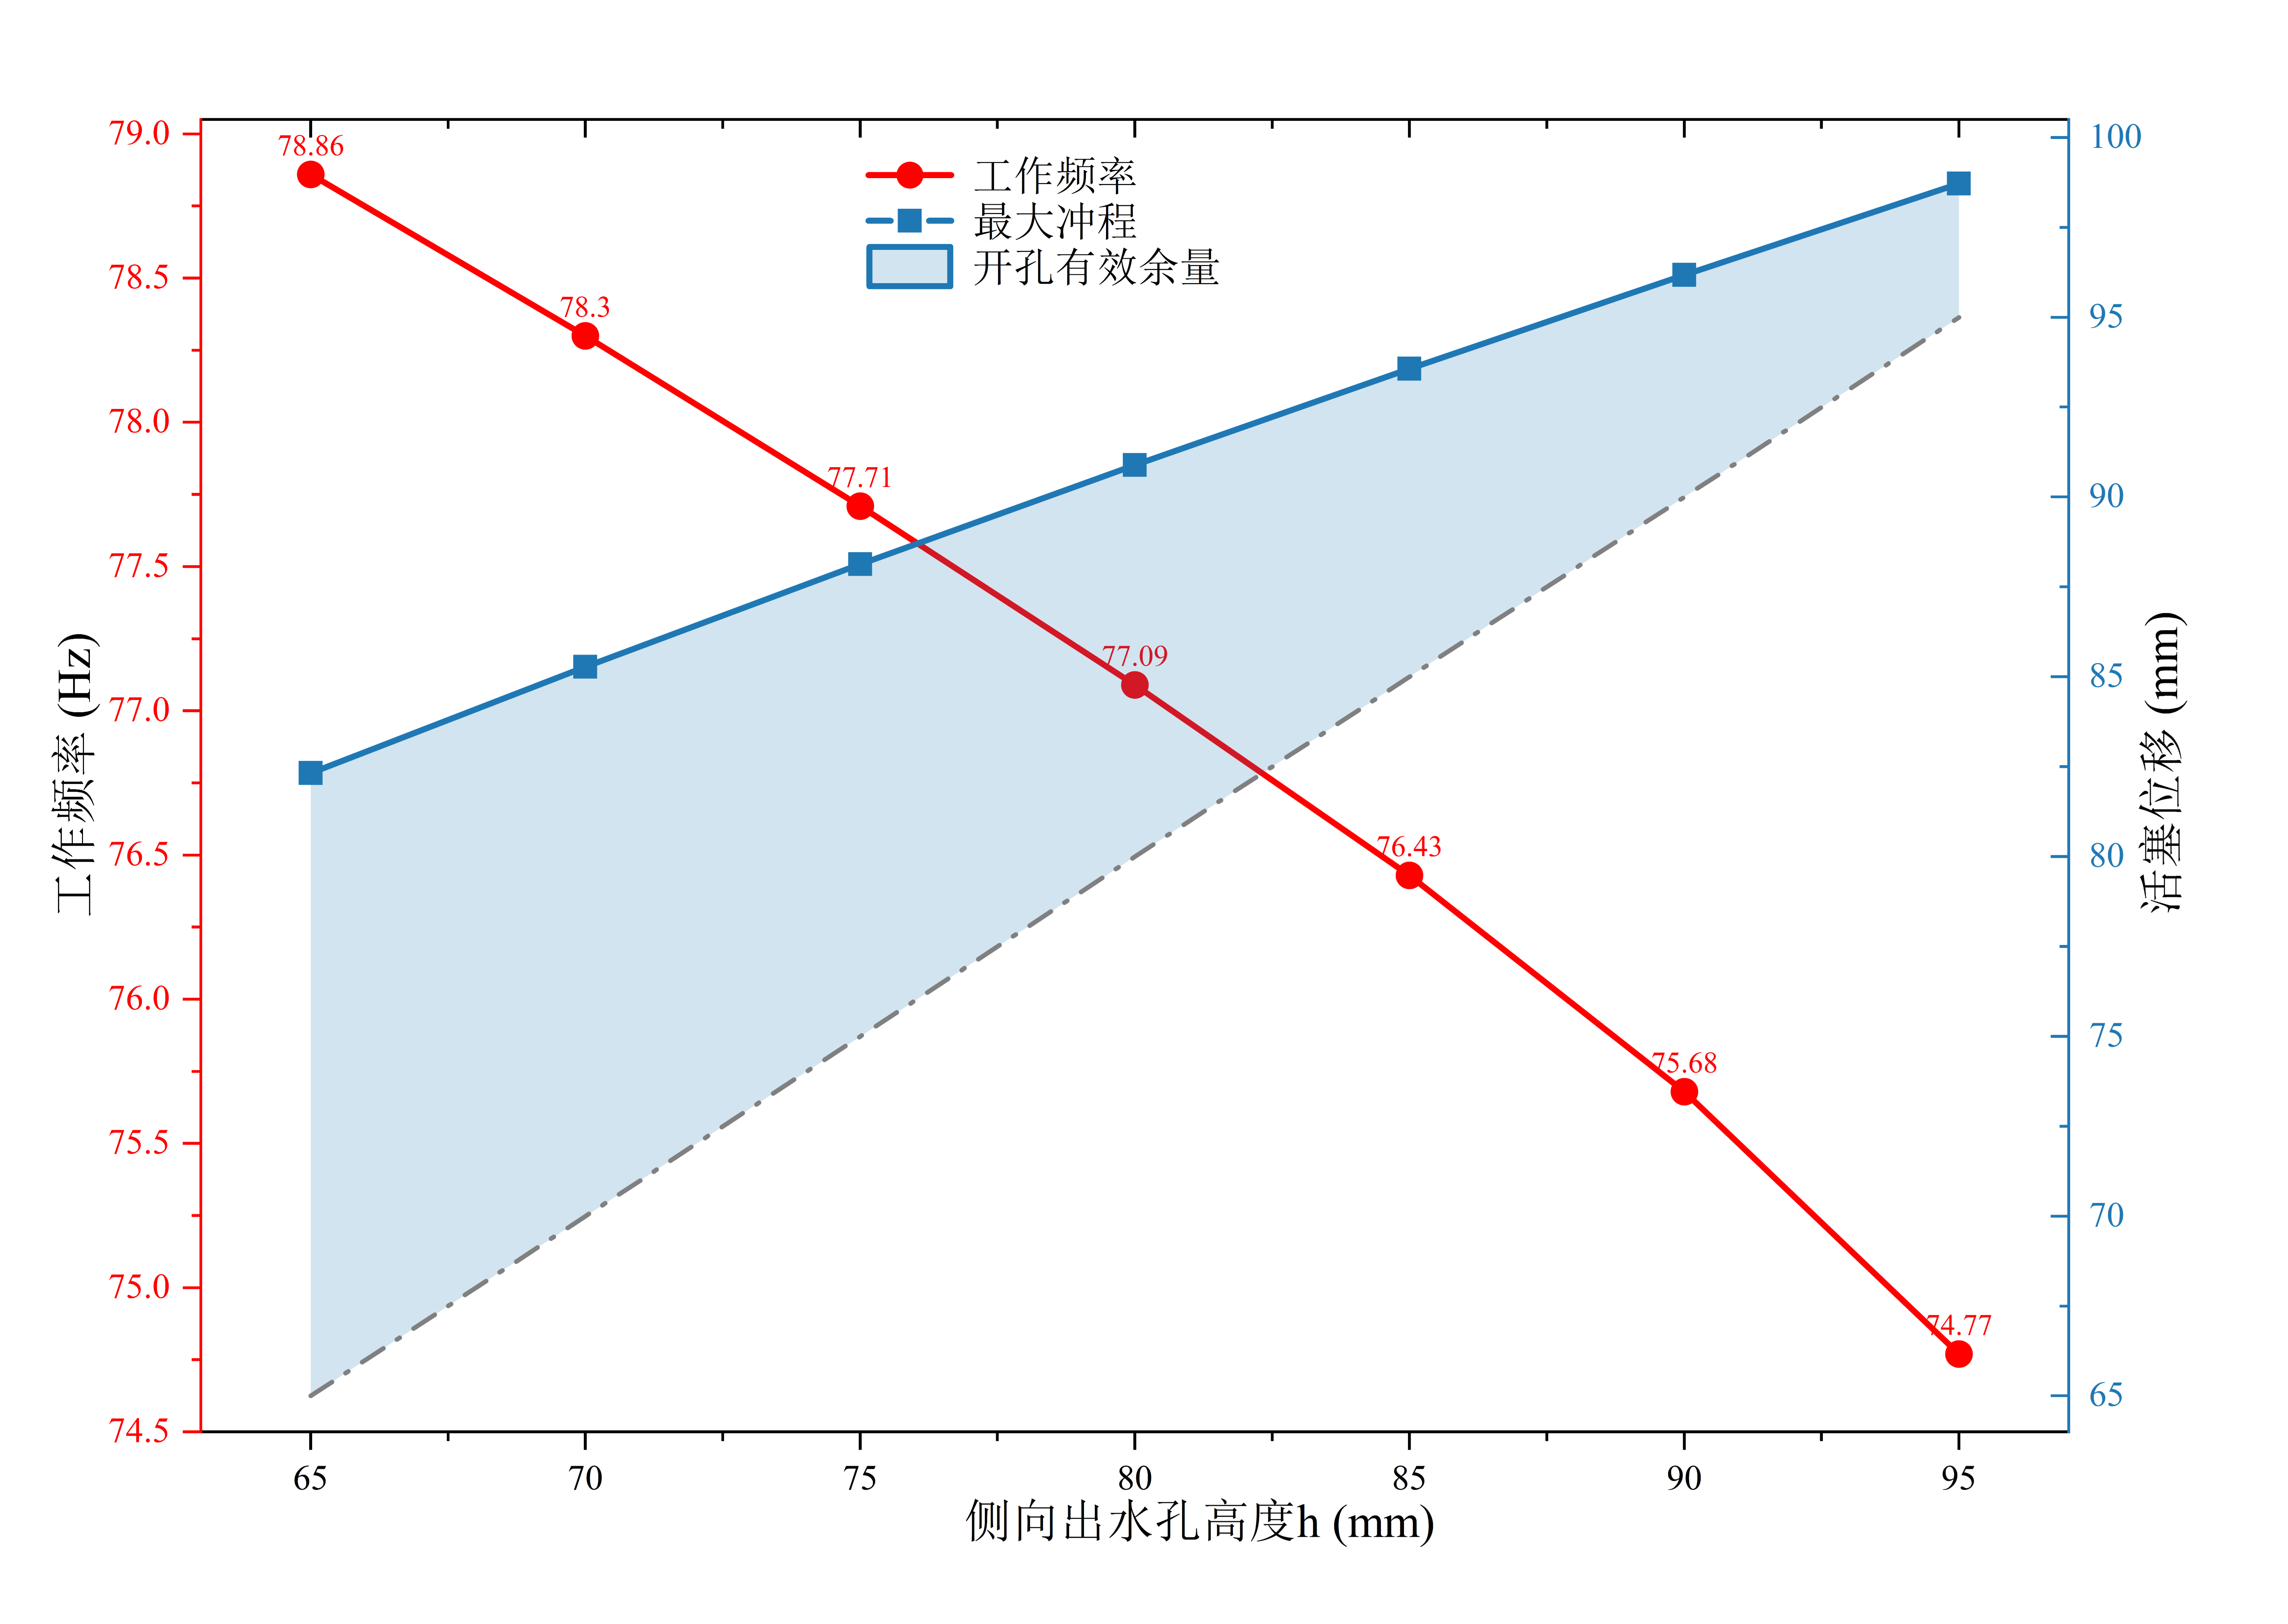
\includegraphics[width=0.7\textwidth]{figure/chapter3/piston-frequency-stroke-VS-h.png}
	\caption{侧向出水孔高度$h$对工作频率与冲程的影响特征曲线}
	\label{fig:piston_frequency_stroke_VS_h}
\end{figure}

\subsection{水力脉冲冲砂洗井工具下砂砾运移仿真分析}
在上一小节中，本文对脉冲冲砂洗井工具进行结构设计以及动力学特性进行研究，成功建立了脉冲发生模块的瞬态动力学数学模型，并深入研究了输入排量$Q$、工具矩形弹簧刚度$K$、工具侧向出水孔高度$h$等核心参数对系统频率与冲程的影响规律。

本小节通过FLUENT软件对使用脉冲冲砂洗井工具下环空井眼的清洁进行数值模拟，对比分析有无工具对环空内砂砾质量的影响，评估脉冲冲砂洗井工具冲砂洗井的效率优势。

\subsubsection{脉冲发生模块的网格划分与边界条件}
井筒内壁尺寸$244.475\mathrm{mm}$，钻杆尺寸$88.9\mathrm{mm}$，井筒长度$1.5\mathrm{m}$，在此基础上，对脉冲发生模块的井筒环空几何模型进行网格划分。如图\ref{fig:pulser_mesh}所示，总体使用poly-hexcore网格划分，网格总数105786，网格质量0.9。

\begin{figure}[htbp]
	\centering
	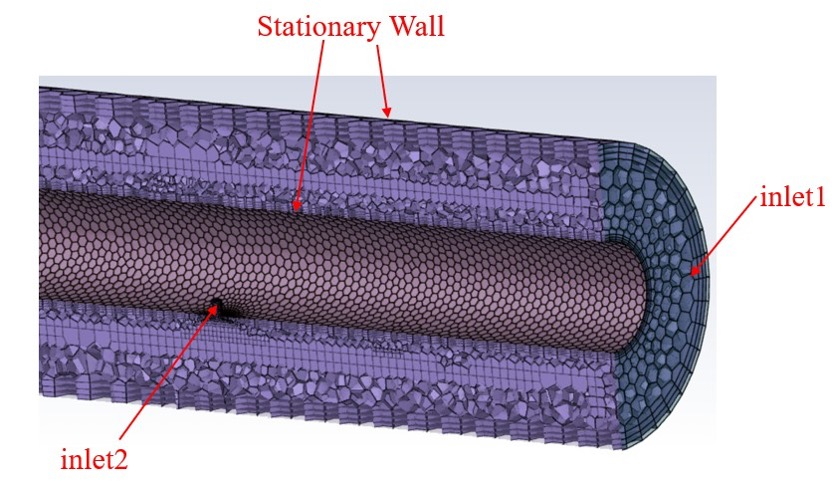
\includegraphics[width=0.7\textwidth]{figure/chapter3/pulser-mesh.jpg}
	\caption{使用水力脉冲冲砂洗井工具的网格划分}
	\label{fig:pulser_mesh}
\end{figure}

根据实际工况，数值模型的入口边界条件定义为冲砂液速度入口和砂砾的颗粒质量入口inlet1；喷嘴处的入口边界条件定义为冲砂液速度入口inlet2；出口的边界条件定义为压力出口outlet；井壁和钻杆内壁面的边界条件定义为固定无滑移的Stationary Wall，具体参数如表4.1所示：

%这里缺少表4.1

脉冲发生模块的侧向出水孔为直径$D=8\mathrm{mm}$的圆孔。设活塞在$t$时刻的位移为$x(t)$，基准开启高度$l_1=75\mathrm{mm}$，则圆孔的瞬时裸露高度$h(t)=\min(y(t)-l_1,D)$。根据微积分弓形面积公式，瞬时开孔面积$A_{\mathrm{out}}(t)$与瞬时射流速度$V_{\mathrm{out}}(t)$遵循以下耦合方程[70]：

%这里缺少公式4.29
其中，$V_p(t)$为活塞瞬时速度，$\mathrm{m/s}$。结合以上喷射时间和喷射速度，通过Fluent读取UDF文件产生周期性的脉冲射流。

\subsubsection{水力脉冲冲砂洗井工具对携砂效率的影响}
为了对比有无脉冲冲砂洗井工具对井筒除砂效率的影响，需设置一组无脉冲冲砂洗井工具的对照组仿真，其它参数保持一致。有脉冲冲砂洗井工具组喷嘴位于钻杆入口$0.4\mathrm{m}$处。通过Fluent欧拉多相流计算井筒内的砂砾质量随时间的变化规律，对比无脉冲洗井工具对照组的砂床运移效率。从图\ref{fig:sand_mass_in_annular_VS_time_pulser_rigid}可以看出，使用脉冲冲砂洗井工具的砂砾质量比无脉冲洗井工具对照组降低了19\%，该工具可以明显提升砂砾运移效率[71-72]。

\begin{figure}[htbp]
	\centering
	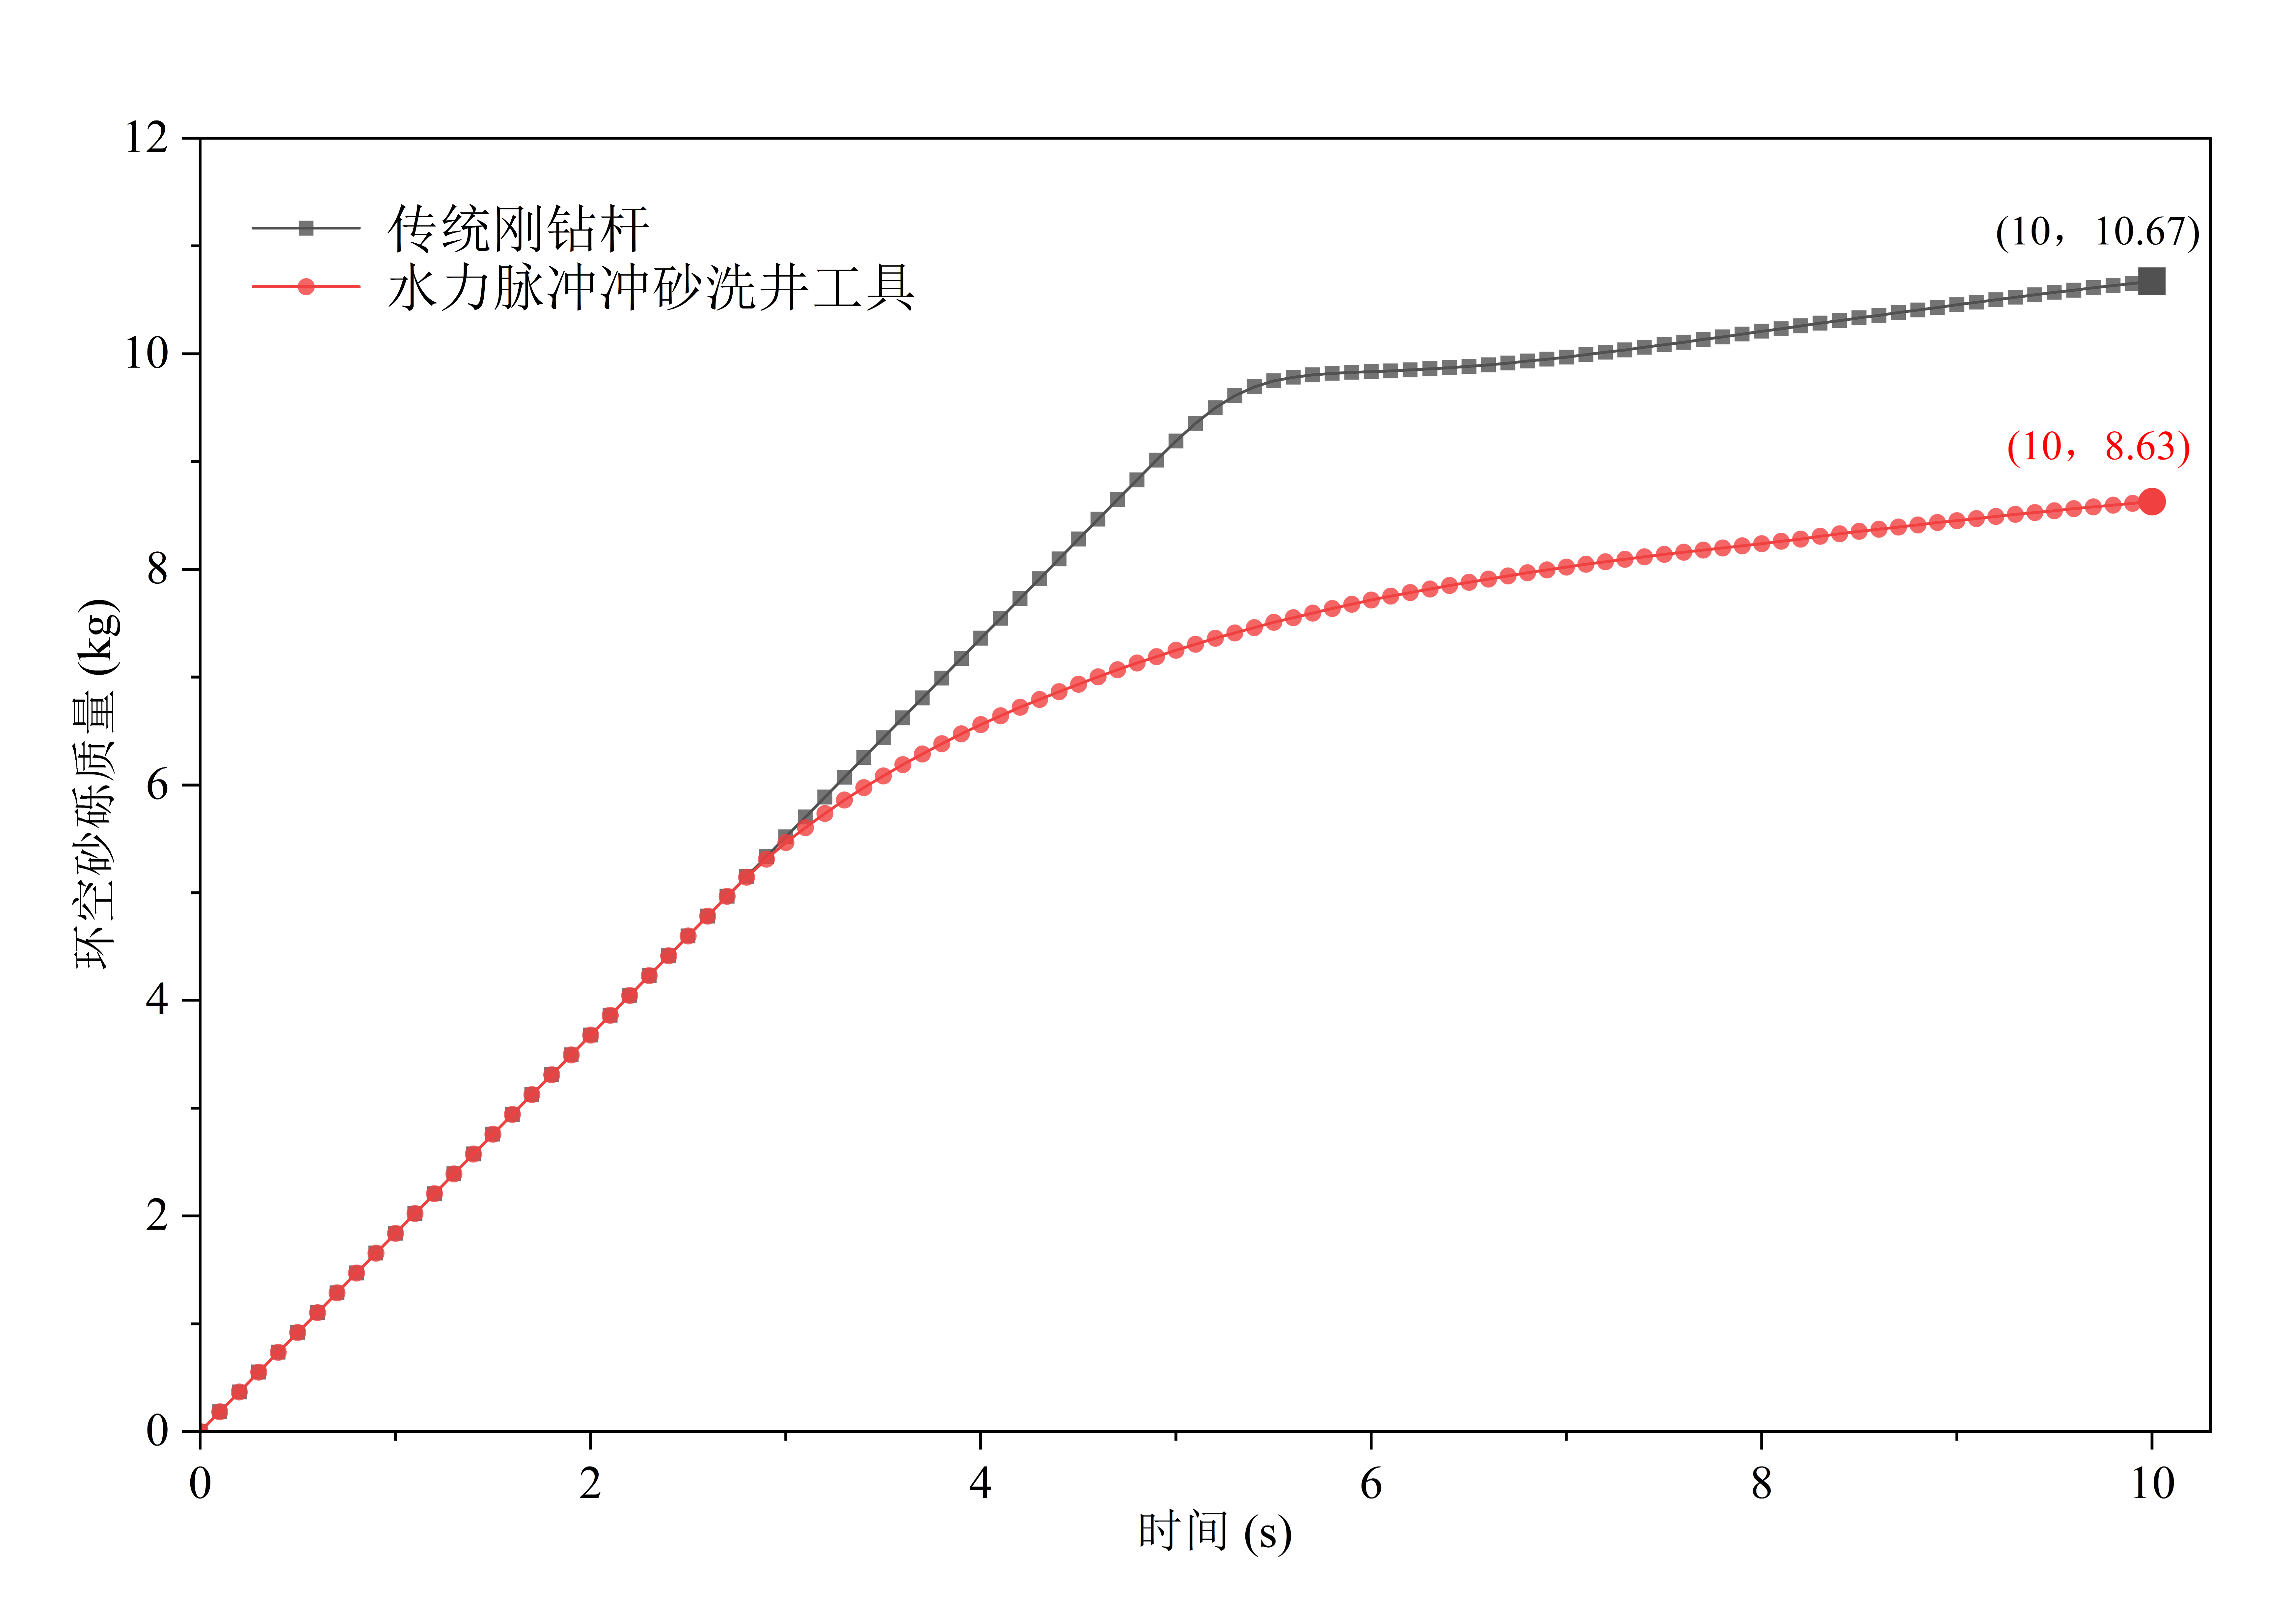
\includegraphics[width=0.7\textwidth]{figure/chapter3/sand-mass-in-annular-VS-time-pulser-rigid.png}
	\caption{环空砂砾质量变化对比图}
	\label{fig:sand_mass_in_annular_VS_time_pulser_rigid}
\end{figure}

图\ref{fig:axial_velocity_near_nozzle_section}为喷嘴截面处冲砂液轴向速度对比图，带有工具的截面环空下方冲砂液轴向速度明显高于传统刚钻杆环空下方的冲砂液轴向速度，这说明带有脉冲喷嘴的钻杆可以有效提高冲砂液的携砂能力，使砂砾的运移效率显著提高。
\begin{figure}[htbp]
	\centering
	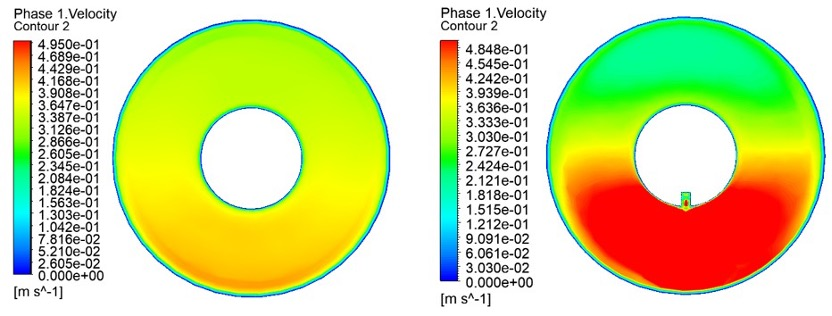
\includegraphics[width=0.7\textwidth]{figure/chapter3/axial-velocity-near-nozzle-section.jpg}
	\caption{喷嘴截面处冲砂液轴向流速对比图}
	\label{fig:axial_velocity_near_nozzle_section}
\end{figure}

图\ref{fig:sand_volume_at_nozzle_section}为相同时刻下喷嘴截面处有无工具砂砾体积分数对比图，从图中可以看出，使用传统刚钻杆仿真组的砂砾会在环空底部发生沉积，使用水力脉冲冲砂洗井工具仿真组的砂砾由于脉冲喷嘴的冲击压力并未沉积在环空底部，而是富集于环空两侧，富集区域最大体积分数远小于传统刚钻杆仿真组。

\begin{figure}[htbp]
	\centering
	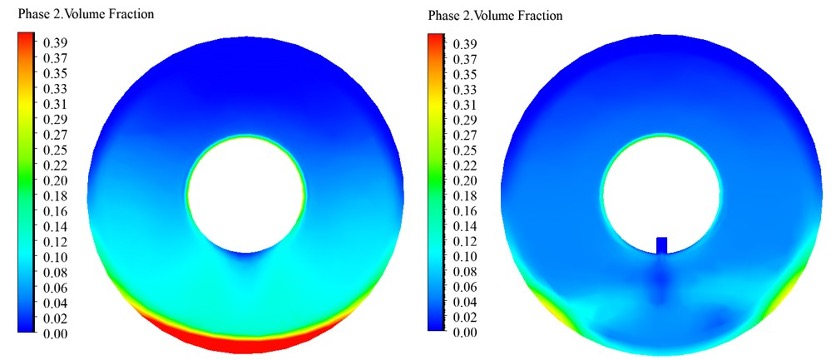
\includegraphics[width=0.7\textwidth]{figure/chapter3/sand-volume-at-nozzle-section.jpg}
	\caption{喷嘴截面处冲砂液轴向流速对比图}
	\label{fig:sand_volume_at_nozzle_section}
\end{figure}


图\ref{fig:sand_volume_at_verticle_section}为相同时刻下环空有无工具砂砾体积分数对比图，从图中可以看出，使用传统刚钻杆仿真组的砂砾从入口处进入环空后迅速在环空底部发生沉积，并形成连续砂床。砂床右端运移到距离入口0.8m处。使用水力脉冲冲砂洗井工具仿真组的砂砾从入口处进入环空并开始沉积，当砂砾运移到脉冲喷嘴处时会被脉冲喷嘴产生的冲击压力与负压抽吸效果重新卷积到井筒环空中，并在脉冲喷嘴下游处沉积，砂床右端已运移到压力出口。可以发现，使用工具可以有效抑制砂砾在工具处的沉积现象，并且显著提升砂床的运移效果。

\begin{figure}[htbp]
	\centering
	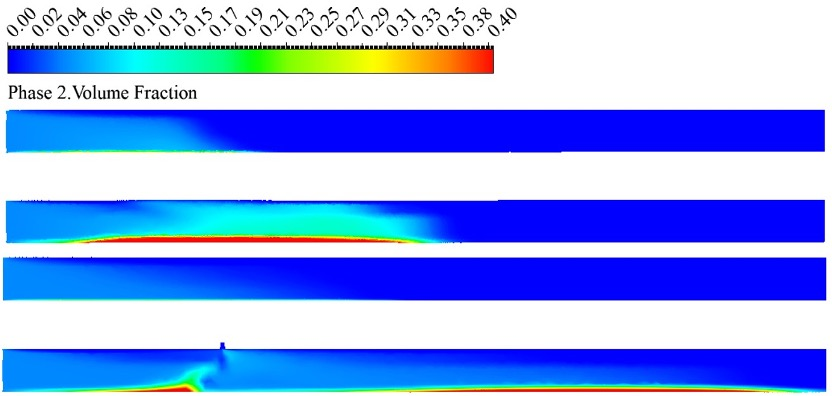
\includegraphics[width=0.7\textwidth]{figure/chapter3/sand-volume-at-verticle-section.jpg}
	\caption{喷嘴截面处冲砂液轴向流速对比图}
	\label{fig:sand_volume_at_verticle_section}
\end{figure}

\subsection{水力脉冲喷头流动仿真}
\subsubsection{水力脉冲计算域的构建与离散}

为了定量研究清洁工具产生的脉冲射流的清洁作用，需建立流动模型，采用流体动力学方法进行研究。在建立流动模型过程中，考虑到工具的外部表面平滑（如图3.1(a)所示），且水力脉冲对井筒的影响的窗口是喷嘴，为了研究脉冲频率的影响，依据隔离法的思想，可将研究对象选为喷嘴以外的环空区域，所构建的流体域如图\ref{fig:pulsing_nozzle_sub_model}(a)所示。
在网格划分采用多面体网格进行划分，能产生更多的邻居单元，能够更精确地计算控制体的梯度，在边界附近增加三层边界层以捕获准确的流动特征，提高计算准确度和精度。另外对流道差异转化较大的区域进行局部加密，优化网格质量，并进行网格无关性验证，最终的离散结果如图\ref{fig:pulsing_nozzle_sub_model}(b)所示。
\begin{figure}[htbp]
	\centering
	\subfloat[水力脉冲清洁工具流体域构建]{%
	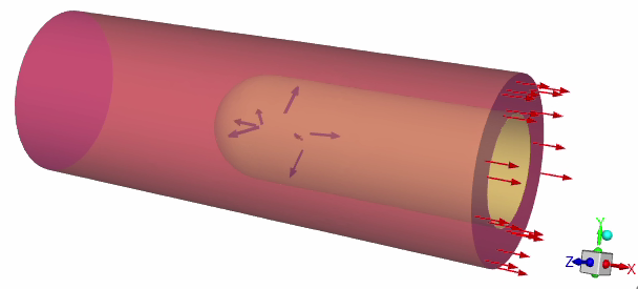
\includegraphics[width=0.45\textwidth]{figure/chapter3/nozzle-sub-fluid-domain.png}
	}
	%\vspace{1em}
	\subfloat[环空流体域的多面体离散结果]{%
	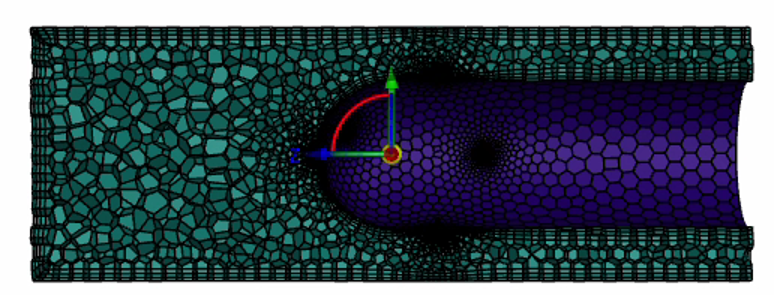
\includegraphics[width=0.45\textwidth]{figure/chapter3/nozzle-sub-fluid-domain-mesh.png}
	}
	\caption{水力脉冲喷头计算模型}
	\label{fig:pulsing_nozzle_sub_model}
\end{figure}


边界条件设置如下：出口假设为套管轴向内测，该设置对流场及仿真结果无影响，且避免了回流的影响，出口为压力出口，压力大小为大气压；入口边界条件设置为速度入口，该速度入口采取$25-45m^3/h$的动态范围脉动流量的转化量进行设置，该结构共设置7组喷嘴，每个喷嘴的尺寸直径为$\phi 3.25$，转化后的入口速度$v$为
\begin{equation}
	v=60.63 \sin⁡(2\pi/Tt)+262.73
\end{equation}

为研究脉动频率对压力的作用情况和井筒的清洁效果分别开展以下三组实验：$T=0.5s$、$1.0s$或$2.0s$。仿真采用的瞬态流动求解器，时间步长$0.001s$，初始流场的速度和压力置零。

\subsubsection{仿真结果及讨论}

为正确反应该水力脉冲清洁工具的清理能力，以冲击点的压力波动为因变量进行分析，$t=0.5s$时套管内壁面的压力分布如图\ref{fig:sress_distribution_at_case}所示。图\ref{fig:case_wall_pressure_t_dot5s}显示流体冲击作用对应下的近壁面压力最高，压力呈圆周状进行削减。图\ref{fig:case_wall_shear_t_dot5s}说明高速射流在壁面附近形成强烈的速度梯度，圆孔射流冲击壁面后形成径向流动，剪切应力由流体在壁面附近的黏性摩擦产生。剪切应力沿径向分布，能够扩大清洗覆盖范围，这种应力会克服污染物与管壁之间的黏附力，从而剥离附着物。高速射流带动周围流体形成涡流，使得流道内湍流强度较高，其瞬时脉动会增强剪切力的波动性，更有效地破坏污染物的结构，使剥离的污垢颗粒被卷吸进入主流，防止重新沉积。

\begin{figure}[htbp]
	\centering
	\subfloat[正压力]{%
	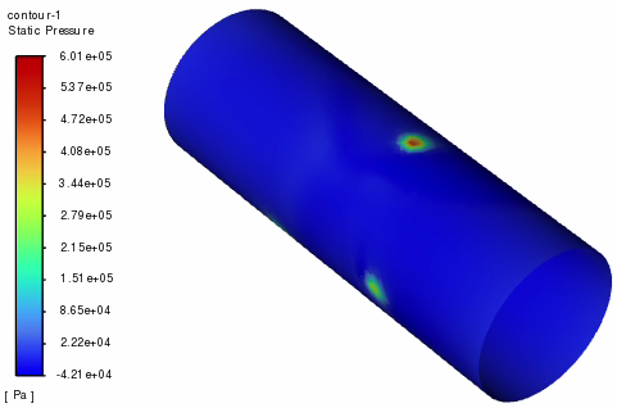
\includegraphics[width=0.45\textwidth]{figure/chapter3/case-wall-pressure-t-dot5s.png}
	\label{fig:case_wall_pressure_t_dot5s}
	}
	\vspace{1em}
	\subfloat[剪切应力分布]{%
	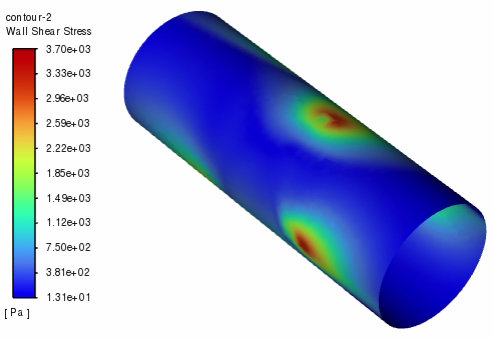
\includegraphics[width=0.45\textwidth]{figure/chapter3/case-wall-shear-t-dot5s.png}	\label{fig:case_wall_shear_t_dot5s}
	}
	\caption{水力脉冲喷头作用下套管内壁压力分布（$t=0.5s$）}
	\label{fig:sress_distribution_at_case}
\end{figure}

整个过程中，冲击压力与剪切应力协同起作用。射流的冲击压力首先使污染物破裂或松动，后续产生的持续的剪切应力将已松动的污染物卷吸进入流体主流，并随流道被带走，达到清洁壁面的目的。流体在流道内的速度流线图如图\ref{fig:nozzle_streamline_dot5s}所示。该图显示喷嘴孔射流流速逐渐减小，动压增大，并逐渐转化为静压作用于油管壁面或清理面，射流压力是影响清垢效率的一个重要因素，在其它条件不变的情况下,随着压力的增加，清垢效率明显提高。该过程通过压力变化反应了水力脉冲清洁工具的清理能力。同时由于射流方向与出口的关系，流场出现许多绕流，该绕流能从各个方向上作用于结垢物上，提升清理能力。

\begin{figure}[htbp]
	\centering
	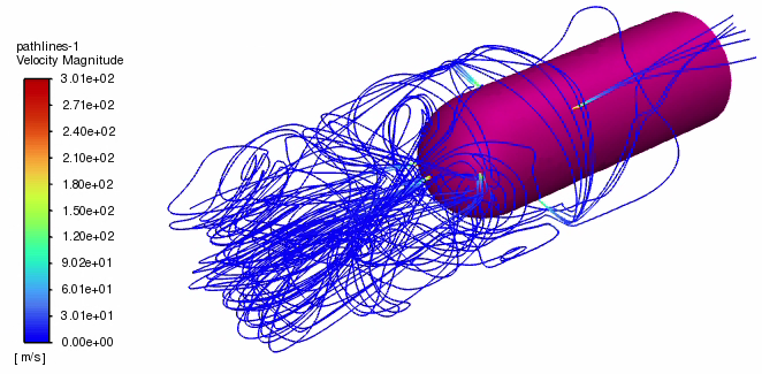
\includegraphics[width=0.7\textwidth]{figure/chapter3/nozzle-streamline-dot5s.png}
	\caption{喷嘴处速度流线图}
	\label{fig:nozzle_streamline_dot5s}
\end{figure}

为研究水力脉冲与压力脉动的关系，将图3.5显示的压力最高点设置为监测点，也就是每个喷嘴作用于井筒的直线冲击点作为监测点，共设置如图\ref{fig:monitoring_point_configuration}所示的6个监测点。当$T=0.5s$、$1.0s$和$2.0s$时，6个监测点对应的壁面压力随时间变化如图\ref{fig:monitoring_points_pressure_T_dot5s}至\ref{fig:monitoring_points_pressure_T_2s}所示。

\begin{figure}[htbp]
    \centering
    % 子图 (a)
    \subfloat[监测点设置]{%
        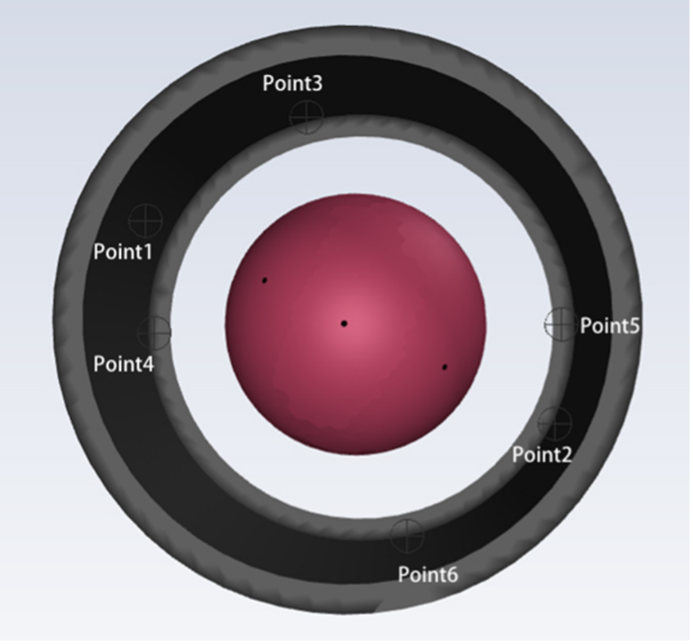
\includegraphics[width=0.4\linewidth]{figure/chapter3/monitoring-point-configuration.png}%
        \label{fig:monitoring_point_configuration}
    }
    % 子图 (b)
    \subfloat[$T=0.5s$]{%
        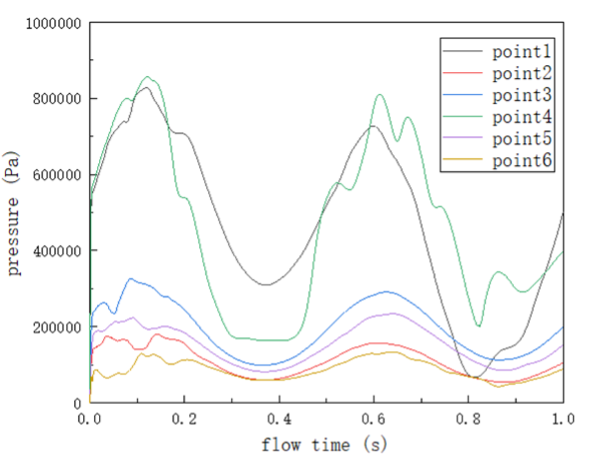
\includegraphics[width=0.45\linewidth]{figure/chapter3/monitoring-points-pressure-T-dot5s.png}%
        \label{fig:monitoring_points_pressure_T_dot5s}
    }
    \vspace{1em}
     % 子图 (c)
    \subfloat[$T=1.0s$]{%
        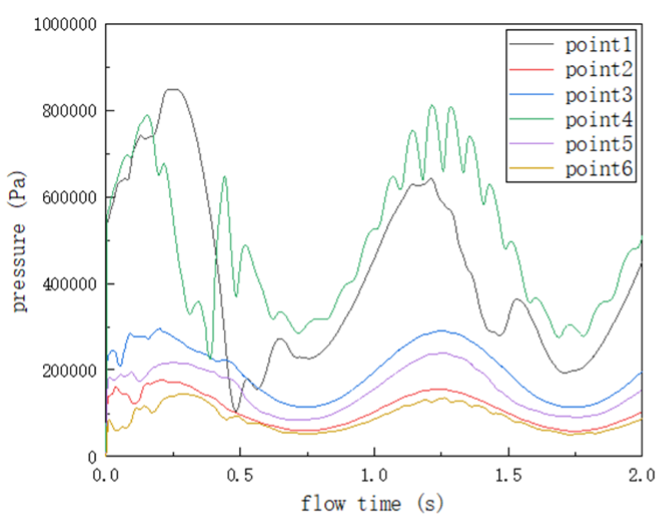
\includegraphics[width=0.45\linewidth]{figure/chapter3/monitoring-points-pressure-T-1s.png}%
        \label{fig:monitoring_points_pressure_T_1s}
    }
    % 子图 (d)
    \subfloat[$T=2.0s$]{%
        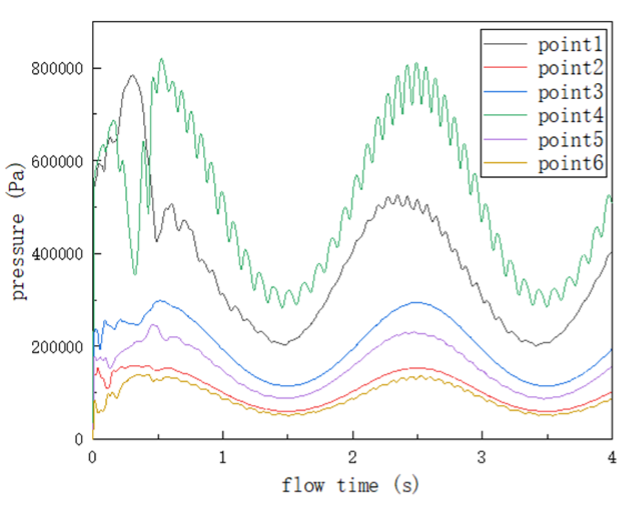
\includegraphics[width=0.45\linewidth]{figure/chapter3/monitoring-points-pressure-T-2s.png}%
        \label{fig:monitoring_points_pressure_T_2s}
    }
        \caption{套管壁面压力点监测结果}
    \label{fig:pressure_at_monitoring_points}
\end{figure}

图\ref{fig:monitoring_points_pressure_T_2s}显示某些监测点的压力较大，压力波动范围更大。由于安装的喷嘴角度不同，若喷嘴射流方向垂直于油管内壁，冲击点会形成驻点（流速降为零，动压转化为静压），导致局部压力显著升高。若射流与壁面存在夹角，高速射流会诱导剪切层分离，形成涡旋结构，这些涡周期性脱落会引发壁面压力剧烈波动，尤其在分离区再附着点附近。另外，由于存在多个射流，射流流场混合导致局部流速增加和压力梯度增强。油管圆柱曲率会改变射流发展路径，凸面曲率可能加速流动分离，进一步加剧压力波动。

随着周期的增加，总体作用点的压力波动幅值于相位保持一致，系统非线性（如边界层分离、射流-壁面相互作用、流道内反射播传播）可能将低频能量传递至高频，生成$4\omega$，$6\omega$等谐波，表现为小幅高频振荡。低频脉动使射流产生间歇性高压冲击，类似于“锤击”效应，适用于硬质或粘附性强的污垢，污垢在反复的低频压力加载下发生微裂纹扩展，最终整体剥离。高频压力波动诱发空化气泡，溃灭时产生局部微射流，直接冲击污垢微结构。高频脉动提升湍流强度（湍动能增加），使剪切应力分布更均匀。另外，观测到部分点高频流速下峰峰值更大，这主要是能量更易耗散，反射叠加效应较弱。

因此，在处理污垢时，压力波动产生的低频和高频成分共同作用，低频脉动剥离大块污垢，高频成分清除残留微粒。叠加高低频脉动，可同时实现宏观剥离和微观清洁。所以实际应用中需根据污垢特性（硬度、厚度、黏附性）调整脉冲频谱，必要时采用复合频率策略以兼顾清洗效率与精度。本章在进行入口脉冲频率选择时需同时考虑压力脉动的组合特性，叠加高低频脉动，以发挥最大的清洁能力。
本章针对连续砂床或严重出砂井况，常规水力冲砂冲砂效率低，除砂效果差的问题，提出并设计了一种新型水力脉冲冲砂洗井工具，能够有效破坏砂床表面并且抑制环空砂砾的再沉积，并对工具进行以下研究：

（1）设计了由旋转喷头模块与脉冲发生模块协同工作的新型水力脉冲冲砂洗井工具。阐述了旋转模块利用偏心射流反冲力矩实现360°冲洗，以及脉冲模块利用往复活塞与弹簧机构将稳态泵注液转化为高频压力脉冲波的工作原理。

（2）对脉冲发生模块进行动力学建模，针对工具内部流体压力与机械部件的耦合机制，基于连续性方程与牛顿运动定律，建立包含蓄能、开启、喷射与复位四个阶段的非线性常微分方程组。通过求解该模型，定量考察了输入排量、矩形弹簧刚度及侧向出水孔高度对活塞冲程与系统工作频率的影响规律，为工具关键物理参数的优选提供数学计算依据。

（3）最后利用Fluent软件模拟脉冲射流动态冲刷下井底沉积砂床的剥离与运移过程，通过对比使用该工具前后的环空携砂质量与流场分布特征，结果显示，使用水力脉冲冲砂洗井工具能够显著提升砂砾的运移效率，实现有效清砂。